\documentclass[uplatex,dvipdfmx]{jsarticle}
\usepackage{url}
\usepackage{longtable}
\usepackage{tabularx}
\usepackage{array}
\usepackage{multirow}
\usepackage{amsmath}
\usepackage{amssymb}
\usepackage{graphicx}
\usepackage{tikz}
\usetikzlibrary{shapes.geometric, arrows.meta, positioning, fit, backgrounds}
\usepackage{pgfplots}
\pgfplotsset{compat=1.18}
\usepackage{algorithm}
\usepackage{algorithmic}
\floatname{algorithm}{アルゴリズム}
\renewcommand{\algorithmicrequire}{\textbf{入力:}}
\renewcommand{\algorithmicensure}{\textbf{出力:}}
\InputIfFileExists{git_revision.tex}{}{%
  \newcommand{\ReportGitCommit}{未設定}%
  \newcommand{\ReportGitTag}{未設定}%
}
\AtBeginDvi{%
  % IPAex TrueTypeをUnicodeで埋め込み、閲覧環境に依存しない日本語表示と
  % 検索・コピーを可能にする（TeX Liveのipaexパッケージを使用）。
  \special{pdf:mapline uprml-h unicode ipaexm.ttf}%
  \special{pdf:mapline uprml-hq unicode ipaexm.ttf}%
  \special{pdf:mapline uprml-v unicode ipaexm.ttf -w 1}%
  \special{pdf:mapline upgbm-h unicode ipaexg.ttf}%
  \special{pdf:mapline upgbm-hq unicode ipaexg.ttf}%
  \special{pdf:mapline upgbm-v unicode ipaexg.ttf -w 1}%
  \special{pdf:tounicode UTF8-UTF16}%
}

\begin{document}

\pagestyle{empty}

\begin{center}
\vspace*{1cm}
\large
{\LARGE 卒業研究報告書}\\
\vspace*{0.8cm}
題目\\
\vspace*{1cm}
\parbox{15.5cm}{\centering\LARGE
収集画像から生成したRTI・部分画像を用いた\\[2mm]
マルチモーダルLLMによるPTP包装識別}\\
\vspace{3mm}

\vspace*{3cm}
指導教員\\
\vspace*{0.3cm}
\underline{\LARGE 森山　真光　准教授}\\
\vspace*{3cm}
報告者\\
\vspace*{0.3cm}

{23--1--211--0009}\\
\vspace*{0.3cm}
\underline{\Huge 呉竹　櫂人}\\
\vspace*{0.5cm}
近畿大学情報学部情報学科\\
\vspace*{2cm}
令和8年7月31日提出\\
\end{center}

\newpage
\normalsize

\clearpage
\begin{center}
{\bf \Large 概要}
\end{center}

薬剤の取り違え防止には，外観が類似するPTP包装を正確に識別する必要がある．
撮影画像だけを学習元とする場合，残存錠数や切り出し範囲を変えた学習用写真を薬剤ごとに個別へ撮影する必要がある．
本研究では，1クラスにつきフルシートの表面1枚と裏面1枚を学習元とし，そこから学習データを構成する方法を検討した．
表裏を結合したRe-oriented Two-sided Image（RTI）と複数サイズの部分画像を生成し，41クラスを対象としてQwen3.5-4Bを
マルチモーダルLLMとしてLoRAで追加学習した．
本研究の目的は，このとき41クラスのPTP包装について，収集画像学習には使用していない近畿大学病院薬剤部で撮影した写真を使い，
Top-1識別性能を評価することである．

本報告書で主結果として扱うver4条件Dは，薬剤部で撮影した評価画像287枚中280枚を正しく識別した．
単剤Top-1精度は97.56\%であった．
同条件の合成複数薬剤画像400枚では，画像単位完全一致率が82.75\%，領域ラベル一致率が95.83\%であった．
結果確認後の探索的追試ver6は286/287（99.65\%）を示した．
ただし，ver6は事後的に選択した条件であり，条件Cとの対応比較で有意差は認められなかった．
また，ver8およびver9のアダプタ，ならびに初期実画像方式の保存済み最良条件でも286/287（99.65\%）が記録されていた．
したがって，ver6が全方式で最も高いことを示す結果ではなかった．
ver8とver9は2経路パッケージであり，その単剤経路は保存済みver6アダプタを用いる設定であった．
条件Cへ適用した信頼ゲートは，回答した既知薬剤134枚をすべて正しく識別した一方，未知薬剤58枚中8枚を既知薬剤として回答した．

追加学習していないQwen3.5-4Bは，41クラスの薬剤名をそのままの形では出力できなかった（厳密一致0/287）．
ただし，追加学習していない側とLoRAを適用した側では入力の前処理と出力の制御が異なるため，この差はLoRAだけの効果ではない．
収集画像42枚の出典も再確認したが，一部の画像は元画像から現存画像までの加工の履歴をたどれなかった．
各学習条件は乱数シード42による1回だけであり，同じ287枚を条件検討に反復使用した．
このため，本研究は41クラスを対象とした識別を実行できることを確認したが，新しい薬剤への一般化，他方式に対する優越性および実用性は確認していない．
学習元をフルシートの表裏2枚へ限定できる構成としたが，収集，撮影および前処理を含む総作業時間は比較しておらず，作業負担の削減量も確認していない．
今後は，対象とする薬剤の数を増やすとともに，間違った薬剤を答えないようにしていく．

\newpage

{\small
\tableofcontents
}
\clearpage
\setcounter{page}{1}
\pagestyle{plain}

%----------------------------------------------------------------------
\section{序論}
%----------------------------------------------------------------------

\subsection{研究背景}

薬剤の取り違えや誤服用は，患者の健康被害につながる医療安全上の課題である．
世界保健機関（World Health Organization：WHO）は，投薬に関連する回避可能な健康被害の削減を国際的な目標としている\cite{who_medication}．
国内でも，調剤時の薬剤取り違えが継続して報告されている\cite{jcqhc_hiyari}．
外観が類似した内服薬の取り違えも分析対象となっている\cite{jcqhc_similarity}．

医療現場では，外箱や薬袋がない状態で薬剤を鑑別する場合がある．
この場合，錠剤の形状，刻印，色，PTP（Press Through Package）包装上の印字などを手掛かりとする．
末次らは，AI画像解析錠剤識別システムを持参薬の一包化鑑別へ導入し，作業時間の短縮とタスク・シフトの可能性を報告している\cite{suetsugu2026ai}．
この報告は，薬剤識別の自動化が薬剤師の負担軽減に寄与し得ることを示している．

\subsection{研究課題}

画像認識モデルを新しい薬剤へ対応させるには，薬剤ごとの学習画像が必要である．
薬剤画像の認識に関する先行研究は，いずれも学習用の薬剤画像データセットを構築したうえで手法を評価している\cite{heo2023pill,radli2024word,radli2024metric}．
撮影画像だけを学習元とする場合，残存錠数，切り出し範囲および向きを変えた学習用写真を薬剤ごとに個別へ撮影する必要がある．
学習画像が不足する場合の一般的な対処としては，幾何変換や色変換によって学習画像の多様性を高める画像拡張が用いられる\cite{shorten2019augmentation}．
そこで本研究では，1クラスにつきフルシートの表面1枚と裏面1枚を学習元とし，そこから派生画像を生成する構成を検討する．
この構成では，残存錠数や切り出し範囲を変えた学習用写真を個別に撮影する必要がない．
ただし，収集画像の取得，出典確認，撮影，背景除去，ラベル確認および前処理に要する時間は方式間で比較していない．
このため，総作業時間または総作業負担の削減量は本研究の評価対象ではない．
本研究で直接検証するのは，収集画像から41クラスの学習集合を構成し，学習には使用していない近畿大学病院薬剤部で撮影した写真について，41クラスの中から薬剤名を答えられるかどうかである．

PTP包装には，錠剤本体だけでなく，薬剤名，含量，識別コードなどの文字情報が含まれる．
一方，表面と裏面では得られる情報が異なる．
片面だけを学習すると，撮影面が変わった場合に識別根拠が不足する．
また，フルシートだけを学習すると，切り分けられたPTP包装や一部だけが写る画像へ対応しにくい．

\subsection{研究目的と提案}

本研究の目的は，収集したPTP包装のフルシート表面・裏面画像からRTIおよび部分画像を生成し，Qwen3.5-4BをLoRAで追加学習することである．
そのうえで，41クラスのPTP包装について，収集画像学習には使用していない近畿大学病院薬剤部で撮影した写真を使い，Top-1識別性能を評価する．
モデルは，あらかじめ定めた41クラスの中から薬剤名を答える．
単剤評価に用いるのは，近畿大学病院薬剤部で撮影した287枚である．
この287枚は，収集画像学習ver1からver9のLoRA学習には使用していない．
ただし，同じ287枚を収集画像学習の条件検討へ反復使用した．
また，研究初期の実画像方式では，この集合の一部を学習にも用いた．
このため，条件を決めた後に新しく撮影した写真での確認は行っていない．

本報告書では，画像と質問文を入力し，薬剤名を文字列として生成するQwen3.5-4Bを，マルチモーダルLLMとして扱う．
視覚言語モデル（Vision-Language Model：VLM）との関係は\ref{sec:vlm}節で述べる．
提案手法は，表裏のフルシート収集画像を正規化する．
次に，表裏を結合したRTIと複数の大きさの部分画像を生成する．
これらの画像へ各実験条件で定めた撮影変動を適用し，マルチモーダルLLMをLoRAで追加学習する．
評価では，収集画像学習には使用していない，近畿大学病院薬剤部で撮影した単剤画像を用いる．
主指標は単剤Top-1精度とWilson法による95\%信頼区間とする．
加えて，誤分類の組合せを列挙する．

本研究で直接評価するのは，単剤Top-1精度，合成複数薬剤画像の画像単位完全一致率と領域ラベル一致率，条件間の画像別正誤対応，追加学習していないQwen3.5-4Bとの比較，Gemini保存予測との比較，および条件Cの信頼ゲートによる予備評価である．
一方，新しい薬剤への一般化，臨床利用可能性，総作業時間の削減量，RTIと部分画像の個別寄与，実写複数薬剤の実用性能，および未知薬剤に対する安全性の確立は，直接評価していない．

本報告書では，検証課題を次の5つに分ける．
\begin{enumerate}
  \item 本報告書で主結果として扱うver4条件Dが，薬剤部で撮影した評価画像でどの程度の識別性能を示すか．
  \item 条件CからLoRAランクを増やしたver6で観測値がどう変化するか（探索的追試）．
  \item 合成複数薬剤画像および黒い区切りのない予備画像で，検出と識別がどこまで成立するか（探索的副次評価）．
  \item 条件Cへ適用した信頼ゲートが，未知薬剤への回答を安全に保留できるか（探索的安全性評価）．
  \item 追加学習していないQwen3.5-4B，保存済みGemini 3.5 Flash予測とLoRA条件の正誤対応がどう異なるか（探索的比較）．
\end{enumerate}

本研究の課題，解決策，評価方法の関係を表\ref{tab:research_summary}に示す．
課題に対し，少数の収集画像を複数の学習画像へ変換する．
その結果を，学習元とは撮影条件の異なる薬剤部の写真で評価する．

\begin{table}[H]
  \centering
  \caption{研究テーマの課題，解決策，評価方法}
  \label{tab:research_summary}
  \small
  \begin{tabular}{|p{2.0cm}|p{10.5cm}|}
    \hline
    項目 & 内容 \\ \hline
    課題 & 薬剤数を増やす際に，残存錠数や切り出し範囲を変えた学習用写真を薬剤ごとに個別へ撮影する必要がある． \\ \hline
    解決策 & 1クラスにつきフルシートの表面1枚と裏面1枚からRTIと部分画像を生成し，画像拡張を用いてマルチモーダルLLMをLoRA学習する． \\ \hline
    評価方法 & 近畿大学病院薬剤部で撮影し，収集画像学習には使用していない287枚について，単剤Top-1精度，Wilson法による95\%信頼区間，誤分類一覧を示す．合成複数薬剤画像は副次評価とする． \\ \hline
  \end{tabular}
\end{table}

本研究は，あらかじめ定めた41クラスの中から薬剤名を答える識別を対象とする．
錠剤そのものを対象とする鑑別全般や，41クラス以外の薬剤が入力される場合の識別は対象としない．
診断，処方，服薬指示には用いず，医療従事者による確認を伴わない臨床利用も対象としない．
また，未知薬剤に対する信頼ゲートは予備評価であり，安全性が確立した機構として扱わない．

\subsection{本報告書の構成}

第\ref{sec:related}章では，薬剤識別，VLMおよびマルチモーダルLLM，LoRA，画像拡張，未知入力の保留に関する研究を整理する．
第\ref{sec:method}章では，収集画像から学習データを生成する手法と評価方法を示す．
第\ref{sec:results}章では，初期実画像方式から収集画像学習ver1からver5までの経緯と，本報告書で主結果として扱うver4条件Dの結果を示す．
続いて，ver6・ver7の探索的追試とver8・ver9の単剤評価，追加学習していないQwen3.5-4BおよびGemini 3.5 Flashとの比較，合成複数薬剤評価，条件Cへ適用した信頼ゲートの補足結果，ならびに実画像に基づく誤分類分析を示す．
第\ref{sec:conclusion}章では，得られた結論と今後の課題を述べる．

\clearpage

%----------------------------------------------------------------------
\section{関連研究・関連技術}\label{sec:related}
%----------------------------------------------------------------------

\subsection{薬剤画像の認識}

Heoらは，錠剤の刻印，形状，色，剤形を認識し，薬剤データベースを検索する手法を提案している\cite{heo2023pill}．
同手法は，刻印検出，外観特徴の認識，文字列補正，候補検索を組み合わせる．
識別モデルの学習に含まれない薬剤でも，データベースに外観特徴と薬剤情報が登録されていれば検索候補にできる．
一方，データベースにも未登録の薬剤を同定できることを意味するものではなく，複数の専用モデルを構成する必要もある．
刻印が不鮮明な場合には，検索に用いる情報が不足する可能性がある．

Rádliらは，薬剤画像の特徴と薬剤説明文の単語埋め込みを組み合わせている\cite{radli2024word}．
さらに，視覚的手掛かりとテキスト情報を用いるメトリクス学習を提案している\cite{radli2024metric}．
Rádliらは，薬剤ごとに異なる説明文の意味情報と画像特徴を学習へ用いている．
一方，本研究のテキスト入力は，全画像に共通するタスク指示であり，薬剤固有の説明情報を与えるものではない．
本研究は，画像と共通質問文を単一のマルチモーダルLLMへ入力し，対象クラス名を文字列として生成する点で異なる．

Menahaらは，Google Geminiを用いた薬剤識別支援システムを提案している\cite{menaha2024gemini}．
生成AIを薬剤画像へ適用する点は本研究と近い．
ただし，同研究は外部サービスを用いるプロンプト型の手法である．
本研究は，重みを取得可能なモデルを薬剤画像で追加学習する．
ただし，本研究では学習と推論をいずれもGPU計算機上で実行しており，端末上での動作は評価していない．

Hanらは，PTP包装の表面と裏面を専用の撮影装置で同時に撮影し，向きと大きさを正規化した両面画像であるRTIを畳み込みニューラルネットワークへ入力する手法を提案した\cite{han2021blister}．
原論文の比較実験では，表面，裏面およびRTIを同じ識別器群へ入力し，RTIで高いF1値を報告した．
本研究は，この両面統合という着想をRTIとして採用する．
一方，Hanらは上下2台のカメラを備えた専用装置を前提とし，包装全体の外形が得られることを想定している．
本研究は，専用装置を用いず，収集画像と部分的なPTP包装画像も対象とする点で異なる．
Hanらは各片面を448 $\times$ 224画素へ正規化し，左右結合後のRTIを448 $\times$ 448画素としたうえで，識別器入力を224 $\times$ 224画素へ変換した．
本研究は左右結合後の画像を448 $\times$ 448画素へ直接リサイズするため，結合前の縦横比を保持していない．

\subsection{Vision-Language Modelとマルチモーダル\mbox{LLM}}\label{sec:vlm}

画像とテキストを同一モデルで扱う手法は，一般に視覚言語モデル（Vision-Language Model：VLM）と呼ばれる．
本報告書では，このうち大規模言語モデルを基盤とし，画像と質問文を入力して文字列を生成するものをマルチモーダルLLMと呼ぶ．
関連研究の一般名称としてはVLMを用い，本研究が追加学習する対象を指す場合はマルチモーダルLLMを用いる．

Baiらは，画像とテキストを統合して扱うQwen-VLを提案している\cite{bai2023qwenvl}．
Qwen-VLは，視覚的質問応答，画像中の文字読み取り，物体位置の理解を扱う．
Qwen3-VLでは，視覚理解と文書理解がさらに拡張されている\cite{qwen3vl2025}．
PTP包装では，文字情報と外観情報の双方が識別手掛かりとなるため，両者を同一モデルで扱えるマルチモーダルLLMを採用する．

本研究では，Qwen3.5-4Bの特定のリビジョンを用いる\cite{qwen35model}．
入力画像に「この錠剤は何という薬ですか？薬剤名だけで答えてください．」という質問を与える．
出力は薬剤クラス名と同じ規則で正規化し，第\ref{sec:method}章に示す文字列一致規則で評価する．

\subsection{LoRAとQLoRA}

LoRA（Low-Rank Adaptation）は，事前学習済みモデルの重みを固定し，低ランク行列を追加学習する手法である\cite{hu2022lora}．
元の重み行列を$W_0 \in \mathbb{R}^{d \times k}$とすると，学習後の変換は式\eqref{eq:lora}で表す．

\begin{equation}
  h = \left(W_0 + \frac{\alpha}{r}BA\right)x,
  \quad
  A \in \mathbb{R}^{r \times k},
  \quad
  B \in \mathbb{R}^{d \times r}
  \label{eq:lora}
\end{equation}

ここで，$x \in \mathbb{R}^{k}$は入力，$h \in \mathbb{R}^{d}$は出力，$r$はランク，$\alpha$は更新量の倍率を調整する係数である．
探索的追試ver6では$r=32$，$\alpha=64$とする．
学習対象には，アテンション層の$q$，$k$，$v$，$o$射影と，MLP層のgate，up，down射影を含める．

QLoRA（Quantized LoRA）は，事前学習済みモデルを4ビットへ量子化し，LoRAを学習する方法である\cite{dettmers2023qlora}．
必要なGPUメモリを削減できる一方で，量子化が対象課題の性能へ与える影響を確認する必要がある．
本研究の条件Aは4ビットQLoRAを用いる．
条件B以降は量子化を行わず，BF16（bfloat16）のLoRAを用いる．

\subsection{画像拡張の関連技術}

画像拡張は，幾何変換や色変換によって学習画像の多様性を高める方法である\cite{shorten2019augmentation}．
PTP包装の撮影では，向きと照明が変化する．
条件Cとver6では，30度刻みの回転12条件と，明度変化5条件を用いる．
主条件Dでは，重複を除いた回転・明度・コントラスト・ガンマ・台形歪み・ぼけ・ノイズの17条件を用いる．
薬剤クラスを維持したまま，撮影時の向き，明るさ，形状および画質の変動を模擬することを目的とする．

\subsection{未知入力の検出と選択的分類}

Hendrycksらは，最大予測確率を用いて誤分類と分布外入力を検出する基準を示している\cite{hendrycks2017ood}．
同時に，分布外入力へ高い確信度を出す場合があることも指摘している．
薬剤鑑別では，未知薬剤を既知薬剤として回答すると危険な誤回答になり得る．

選択的分類は，確信できない入力への回答を保留し，回答率と誤り率を調整する考え方である\cite{geifman2017selective}．
本研究では，この考え方に基づく保留機構を信頼ゲートと呼ぶ．
条件Cへ信頼ゲートを適用した結果は，探索的追試ver6とは異なるアダプタを用い，目的と生成方法も異なるため，安全性に関する補足評価として扱う．

\subsection{本研究の位置付け}

先行研究では，刻印などの専用特徴を認識する方法，画像と説明文を埋め込み空間で照合する方法，外部生成AIを用いる方法が提案されている．
本研究は，収集画像から複数サイズの部分画像を生成し，マルチモーダルLLMを追加学習する．
学習画像とは撮影条件が異なり，収集画像学習には使用していない薬剤部で撮影した評価画像を用いる点に特徴がある．
また，未知薬剤を安全に保留する問題を，識別精度とは分けて扱う．
関連研究と本研究の相違を表\ref{tab:related_comparison}に示す．

\begin{table}[H]
  \centering
  \caption{関連研究と本研究の位置付け}
  \label{tab:related_comparison}
  \small
  \renewcommand{\arraystretch}{1.25}
  \setlength{\tabcolsep}{3.5pt}
  \textbf{（a）対象・入力・手法}\\[1mm]
  \begin{tabularx}{\textwidth}{|>{\raggedright\arraybackslash}p{1.55cm}|>{\raggedright\arraybackslash}p{1.4cm}|>{\raggedright\arraybackslash}X|>{\raggedright\arraybackslash}X|>{\centering\arraybackslash}p{1.25cm}|}
    \hline
    研究 & 対象 & 主な入力 & 手法 & 専用装置 \\ \hline
    Heoら\cite{heo2023pill} & 錠剤 & 錠剤画像 & 刻印・外観認識とデータベース検索 & 不要 \\ \hline
    Rádliら\cite{radli2024word,radli2024metric} & 錠剤 & 薬剤画像と薬剤固有の説明文 & 画像特徴と単語埋め込みによるメトリクス学習 & 不要 \\ \hline
    Menahaら\cite{menaha2024gemini} & 錠剤 & 薬剤画像とプロンプト & 外部サービスのGeminiによる生成 & 不要 \\ \hline
    Hanら\cite{han2021blister} & PTP包装 & 専用装置で撮影した表裏 & RTIと畳み込みニューラルネットワーク & 必要 \\ \hline
    本研究 & PTP包装 & PTP包装の表裏・部分画像と共通質問文 & RTI・部分画像とQwen3.5-4B（マルチモーダルLLM）のLoRA追加学習 & 不要 \\ \hline
  \end{tabularx}

  \vspace{3mm}
  \textbf{（b）未知薬剤への対応と本研究との差}\\[1mm]
  \begin{tabularx}{\textwidth}{|>{\raggedright\arraybackslash}p{1.55cm}|>{\raggedright\arraybackslash}p{3.2cm}|>{\raggedright\arraybackslash}X|}
    \hline
    研究 & 未知薬剤への対応 & 本研究との主な違い \\ \hline
    Heoら\cite{heo2023pill} & データベース検索 & 本研究はマルチモーダルLLMを追加学習し，41クラスの薬剤名を直接生成する． \\ \hline
    Rádliら\cite{radli2024word,radli2024metric} & 原論文で評価なし & 薬剤固有の説明文ではなく，共通質問文を単一のマルチモーダルLLMへ入力する． \\ \hline
    Menahaら\cite{menaha2024gemini} & 評価なし & 重みを取得可能な基盤モデルへLoRA追加学習を行う． \\ \hline
    Hanら\cite{han2021blister} & 評価なし & 専用装置を用いず，収集画像からRTIと部分画像を生成する． \\ \hline
    本研究 & 信頼ゲートを予備評価 & 41クラスに限定し，モデル固定後の新規評価と安全な未知薬剤保留は未完了である． \\ \hline
  \end{tabularx}
\end{table}

表\ref{tab:related_comparison}（a）から，本研究は専用装置を用いず，収集画像と共通質問文をマルチモーダルLLMへ入力する点で先行研究と異なる．
表\ref{tab:related_comparison}（b）から，未知薬剤への対応は予備評価にとどまり，安全な保留を実証したものではない．
また，薬剤固有の説明文を利用するRádliらの方式と，本研究の全画像に共通する質問文は役割が異なる．

\clearpage

%----------------------------------------------------------------------
\section{提案手法}\label{sec:method}
%----------------------------------------------------------------------

\subsection{処理の全体像}

図\ref{fig:pipeline}に，提案手法の処理をUMLのアクティビティ図として示す．
図は「学習側」と「評価側」の2つのスイムレーンに分け，処理の主体と責務の境界を明示する．
黒丸は開始ノード，二重丸は終了ノード，角丸の矩形はアクション，太い横棒はフォークノードおよびジョインノードである．
実線の矢印は制御フロー，破線の矢印はオブジェクトフローを表す．

学習側では，収集した表裏のPTP包装画像を取得して由来を監査し，背景除去と向きの正規化を行う．
続いてフォークノードで制御を分岐させ，RTIの生成と面別部分画像の生成を並行して実行する．
両者はジョインノードで合流し，各実験条件で定めた提示条件による画像拡張を適用したうえで，Qwen3.5-4BをLoRAで追加学習する．
評価側では，収集画像学習に使用していない薬剤部で撮影した評価画像を入力とし，背景除去と448 $\times$ 448画素への正規化を行う．
学習側で得た学習済みLoRAアダプタはオブジェクトフローとして評価側へ渡され，薬剤名の生成に用いられる．
生成した薬剤名を正解ラベルと照合し，Top-1精度と95\%信頼区間を算出して処理を終了する．

\begin{figure}[H]
  \centering
  \begin{tikzpicture}[
    scale=0.82, transform shape,
    act/.style={
      draw, rounded corners=3mm, align=center, text width=3.9cm,
      minimum height=1.0cm, font=\small, fill=blue!6, inner sep=3pt
    },
    pact/.style={
      draw, rounded corners=3mm, align=center, text width=2.95cm,
      minimum height=1.0cm, font=\small, fill=blue!6, inner sep=3pt
    },
    eact/.style={
      draw, rounded corners=3mm, align=center, text width=3.9cm,
      minimum height=1.0cm, font=\small, fill=orange!8, inner sep=3pt
    },
    bar/.style={draw, fill=black, minimum width=5.0cm, minimum height=1.5mm, inner sep=0pt},
    ini/.style={circle, fill=black, minimum size=3.4mm, inner sep=0pt},
    fl/.style={-{Stealth[length=2.6mm]}, thick},
    ofl/.style={-{Stealth[length=2.6mm]}, thick, dashed},
    lane/.style={draw=black!55, thick},
    lanehd/.style={font=\small\bfseries}
  ]
    % --- スイムレーン ---
    \begin{scope}[on background layer]
      \fill[blue!3]   (-3.85, 1.45) rectangle (3.85, -12.00);
      \fill[orange!3] ( 3.85, 1.45) rectangle (11.55, -12.00);
    \end{scope}
    \draw[lane] (-3.85, 1.45) rectangle (3.85, -12.00);
    \draw[lane] ( 3.85, 1.45) rectangle (11.55, -12.00);
    \draw[lane] (-3.85, 0.75) -- (11.55, 0.75);
    \node[lanehd] at (0,     1.10) {学習側};
    \node[lanehd] at (7.70,  1.10) {評価側};

    % --- 学習側 ---
    \node[ini]  (st1) at (0, 0.15) {};
    \node[act]  (a1)  at (0, -1.25) {収集画像の取得と由来監査\\（表面1枚・裏面1枚）};
    \node[act]  (a2)  at (0, -2.85) {背景除去と\\向き正規化 $T(\cdot)$};
    \node[bar]  (fk)  at (0, -3.95) {};
    \node[pact] (a3)  at (-1.85, -5.05) {RTIの生成};
    \node[pact] (a4)  at ( 1.85, -5.05) {面別部分画像の生成};
    \node[bar]  (jn)  at (0, -6.15) {};
    \node[act]  (a5)  at (0, -7.25) {画像拡張\\（提示条件の適用）};
    \node[act]  (a6)  at (0, -8.85) {Qwen3.5-4Bの\\LoRA追加学習};

    \draw[fl] (st1) -- (a1);
    \draw[fl] (a1)  -- (a2);
    \draw[fl] (a2)  -- (fk);
    \draw[fl] (-1.85,-4.03) -- (a3);
    \draw[fl] ( 1.85,-4.03) -- (a4);
    \draw[fl] (a3) -- (-1.85,-6.07);
    \draw[fl] (a4) -- ( 1.85,-6.07);
    \draw[fl] (jn) -- (a5);
    \draw[fl] (a5) -- (a6);

    % --- 評価側 ---
    \node[ini]  (st2) at (7.70, 0.15) {};
    \node[eact] (b1)  at (7.70, -1.25) {薬剤部で撮影した\\評価画像の入力};
    \node[eact] (b2)  at (7.70, -2.85) {背景除去と\\448 $\times$ 448画素への正規化};
    \node[eact] (b3)  at (7.70, -8.85) {薬剤名の生成（貪欲法）};
    \node[eact] (b4)  at (7.70, -10.45) {正解ラベルとの照合と\\Top-1精度の算出};
    \node[circle, draw, thick, minimum size=5.2mm, inner sep=0pt] (fin) at (7.70, -11.75) {};
    \fill (fin.center) circle (1.5mm);

    \draw[fl] (st2) -- (b1);
    \draw[fl] (b1)  -- (b2);
    \draw[fl] (b2)  -- (b3);
    \draw[fl] (b3)  -- (b4);
    \draw[fl] (b4)  -- (fin);
    \draw[ofl] (a6) -- node[above, font=\scriptsize, align=center, pos=0.5, yshift=1pt]
      {学習済みLoRAアダプタ} (b3);
  \end{tikzpicture}
  \caption{提案手法の処理を示すUMLアクティビティ図（スイムレーンで学習側と評価側を分離）}
  \label{fig:pipeline}
\end{figure}

\subsection{収集画像の由来監査}\label{sec:provenance_audit}

薬剤ごとに，PTP包装の表面と裏面を確認できる画像を収集画像として整理する．
採用前に，薬剤名，含量，面の種別，フルシートであるかを目視確認する．
箱だけが写る画像，複数薬剤が混在する画像，極端に低解像度の画像は除外する．
監査項目には，掲載ページURL，画像URL，取得日，表裏の判定を用いる．

由来監査では，現存する収集画像を現行の収集記録と照合する．
直接照合できない画像については，削除前の収集記録まで探索し，掲載ページURLや取得日時から出典記録または出典候補を特定する．
あわせて，収集画像と薬剤部で撮影した評価画像287枚に同一の画像が含まれていないことを確認する．
本監査は保存ファイルと記録行の同一性を確認するものであり，掲載ページの現在の内容，薬剤ラベルの医学的妥当性，利用条件および再配布可否を判定する権利監査ではない．
このため，「出典候補を確認済み」と「加工履歴まで完全に再現可能」を区別する．
収集画像は41クラス・42ファイルであり，1クラスだけが表面と裏面の2ファイルへ分かれる．
監査結果は\ref{sec:data_audit_results}節に示す．
以後，本報告書では，実験管理上の保存名である「Web画像学習」を必要な場合だけ引用し，この学習集合自体は「収集画像」と呼ぶ．

\subsection{RTIと部分画像の生成}

Hanらは，PTP包装の各片面を448 $\times$ 224画素へ向き補正し，左右へ結合した448 $\times$ 448画素の画像をRe-oriented Two-sided Image（RTI）と呼んだ\cite{han2021blister}．
本研究では，この構成に基づく画像をRTIと呼ぶ．
ただし，本研究は結合後の画像を448 $\times$ 448画素へ直接リサイズし，結合前の縦横比を保持しない．
図\ref{fig:rti}にRTIと部分画像の構成を示す．
表面画像$I_{d,f}$と裏面画像$I_{d,b}$から背景を除去する．
PTP包装の凸包を抽出し，透視変換によって向きと大きさをそろえる．
正規化関数を$T(\cdot)$，左右結合を$\Vert$とすると，薬剤$d$のRTIは式\eqref{eq:rti}で表す．

\begin{equation}
  I^{\mathrm{RTI}}_d =
  \operatorname{Resize}_{448 \times 448}
  \left(T(I_{d,b}) \Vert T(I_{d,f})\right)
  \label{eq:rti}
\end{equation}

RTIでは，裏面を左，表面を右へ配置する．
両面を同一画像内に含めることで，片面だけでは不足する文字と外観を同時に提示する．

\begin{figure}[H]
  \centering
  \begin{tikzpicture}[
    panel/.style={
      draw,
      rounded corners=1mm,
      align=center,
      minimum width=3.1cm,
      minimum height=1.55cm,
      font=\small
    },
    process/.style={
      draw,
      rounded corners=2mm,
      fill=orange!12,
      align=center,
      text width=2.6cm,
      minimum height=1.35cm,
      font=\small
    },
    arrow/.style={-{Stealth[length=3mm]}, thick}
  ]
    \node[panel, fill=blue!8] (back) {正規化後の裏面\\$T(I_{d,b})$};
    \node[panel, fill=blue!8, right=0.45cm of back] (front) {正規化後の表面\\$T(I_{d,f})$};
    \node[process, right=0.75cm of front] (join) {左右へ結合};
    \node[panel, fill=green!10, right=0.75cm of join, minimum width=3.8cm] (rti) {RTI\\左：裏面 \quad 右：表面};

    \node[process, below=1.0cm of join] (crop) {固定格子\\縦2分割・縦4分割};
    \node[panel, fill=green!10, right=0.75cm of crop, minimum width=3.8cm] (parts) {面別部分画像\\1錠区画・水平帯};

    \draw[arrow] (back.north) -- ++(0,0.55cm) -| (join.north);
    \draw[arrow] (front) -- (join);
    \draw[arrow] (join) -- (rti);
    \draw[arrow] (front.south) |- (crop.west);
    \draw[arrow] (back.south) |- (crop.west);
    \draw[arrow] (crop) -- (parts);
  \end{tikzpicture}
  \caption{収集画像からRTIおよび面別部分画像を生成する規則の模式図（Hanら\cite{han2021blister}を参考に著者作成）}
  \label{fig:rti}
\end{figure}

\begin{figure}[H]
  \centering
  \includegraphics[width=\linewidth]{figures/generated/actual_rti_pipeline.png}
  \caption[収集元画像および保存済み派生基画像の例]{収集元画像および保存済み派生基画像の例（エンレスト錠200mg）．
  薬剤部で撮影した評価画像ではない．
  （a）収集元の表面，（b）収集元の裏面，（c）正規化後の表面，（d）正規化後の裏面，
  （e）RTI（左：裏面，右：表面），（f）1錠区画，（g）縦2分割，（h）縦4分割である．
  （a）（b）の出典：ノバルティス ファーマ株式会社の製品資料\cite{novartis_entresto_document}．
  （c）から（h）は著者が保存済み実験データから再配置した．}
  \label{fig:actual_rti_pipeline}
\end{figure}

図\ref{fig:actual_rti_pipeline}は，図\ref{fig:rti}の模式的な規則を実際の保存画像へ適用した結果である．
（c）から（h）は再生成せず，ver6の\path{train_manifest.csv}が指す保存済み基画像を用いた．
収集元画像の掲載ページとサイト利用条件\cite{novartis_terms}を確認した．
同条件が引用その他の法令上認められる範囲を示していることを踏まえ，
本図は手法を説明する非営利の学術目的の範囲に限り，出典を明示して掲載する．
公開リポジトリ等へ二次配布する場合は，公開時点の条件と必要な許諾を改めて確認する．

各薬剤では，RTIを1枚生成する．
さらに各面から，フルシート1枚，1錠区画8枚，縦2分割画像2枚，縦4分割画像4枚を生成する．
1錠区画は画像から錠剤セルを自動検出するのではなく，各面の前景外接矩形へ薬剤ごとに定めた固定格子を当て，格子区画に対応する部分画像を左上から行優先で最大8枚生成する．
本実装ではクラス間の基画像数をそろえるため上限を8枚に固定したが，上限値の妥当性を比較する実験は行っていない．
格子の列数と行数は通常の薬剤で$2\times5$，メチコバール錠500$\mu$gで$3\times7$，レボフロキサシン錠500mgで$1\times5$とする．
縦2分割画像と縦4分割画像は，前景外接矩形を高さ方向へ等分した水平帯である．
したがって，この1錠区画の切り出しは既知のPTP配列に基づく固定規則であり，任意の包装に対する一般的な錠剤セル検出器ではない．
通常の薬剤で生成する基画像数$N_d$は式\eqref{eq:base_count}より31枚となる．

\begin{equation}
  N_d = 1 + 2(1 + 8 + 2 + 4) = 31
  \label{eq:base_count}
\end{equation}

レボフロキサシン錠500mgは，PTP包装に含まれる錠剤セル数の制約により1錠区画を5枚とし，式\eqref{eq:base_count_lvfx}の25枚となる．
41クラスについて，クラスごとに1組の収集元画像から派生させた基画像は，式\eqref{eq:base_total}の合計1,265枚となる．

\begin{equation}
  N^{\mathrm{LVFX}}_d = 1 + 2(1 + 5 + 2 + 4) = 25
  \label{eq:base_count_lvfx}
\end{equation}

\begin{equation}
  N_{\mathrm{base}} = 40 \times 31 + 1 \times 25 = 1{,}265
  \label{eq:base_total}
\end{equation}

アルゴリズム\ref{alg:image_generation}に，基画像生成の手順を示す．

\begin{algorithm}[H]
  \caption{収集画像からの基画像生成}
  \label{alg:image_generation}
    \begin{algorithmic}[1]
    \REQUIRE 薬剤$d$の表面画像$I_{d,f}$，裏面画像$I_{d,b}$
    \ENSURE 基画像集合$\mathcal{D}_d$
    \STATE $\mathcal{D}_d \gets \emptyset$
    \STATE 表裏画像から背景を除去し，PTP包装の凸包を抽出する
    \STATE 透視変換により，表裏画像の向きと大きさを正規化する
    \STATE 裏面を左，表面を右へ配置してRTIを生成する
    \STATE 生成したRTIを$\mathcal{D}_d$へ追加する
    \STATE 正規化した表裏フルシートを$\mathcal{D}_d$へ追加する
    \FOR{面$s \in \{f,b\}$}
      \STATE $T(I_{d,s})$の前景外接矩形へ薬剤$d$に対応する固定格子を設定する
      \STATE 格子区画に対応する部分画像を，左上から行優先で最大8枚生成する
      \STATE 前景外接矩形を高さ方向へ2等分し，水平帯を2枚生成する
      \STATE 前景外接矩形を高さ方向へ4等分し，水平帯を4枚生成する
      \STATE 生成画像を$\mathcal{D}_d$へ追加する
    \ENDFOR
    \STATE 各画像を448 $\times$ 448の黒背景へ配置する
    \RETURN $\mathcal{D}_d$
  \end{algorithmic}
\end{algorithm}

\subsection{画像拡張}

主条件Dでは，撮影時の変動を模擬する重複のない17提示条件を用いる．
内訳は，無変換1条件，$\pm15$度，$\pm30$度，90度および180度の回転6条件である．
これに，明度0.7倍と1.3倍，コントラスト0.7倍と1.3倍，ガンマ0.7と1.4，左右の台形歪み，ぼけおよびセンサノイズを各条件として加える．
主条件Dでは，BF16 LoRA，ランク16，スケーリング係数32，
\texttt{q\_proj}，\texttt{k\_proj}，\texttt{v\_proj}，\texttt{o\_proj}，
\texttt{gate\_proj}，\texttt{up\_proj}，\texttt{down\_proj}を対象とし，
5エポックおよび乱数シード42を用いる．

探索的ver6はver4条件Cを基準とする．
条件Cとver6では，回転12条件と明度5条件からなる提示条件$\mathcal{A}_C$を式\eqref{eq:augmentation}で定義する．
回転は0度から330度まで30度刻みとし，明度倍率は0.8，0.9，1.0，1.1，1.2とする．
回転と明度変化は別の提示条件として用いるため，提示数は17となる．
0度回転$R_0$と明度倍率1.0の$B_{1.0}$は画素値が同一だが，実装では別レコードとして1回ずつ提示する．

\begin{equation}
  \mathcal{A}_C
  =
  \left(
    R_{0},R_{30},\ldots,R_{330},
    B_{0.8},B_{0.9},B_{1.0},B_{1.1},B_{1.2}
  \right)
  \label{eq:augmentation}
\end{equation}

図\ref{fig:augmentation_examples}に，主条件Dの17提示条件のうち，回転6条件から4条件と，無変換および明度2条件を抜粋して模式的に示す．
主条件Dでは重複する提示条件を設けないため，画素値を変えない条件は無変換1条件だけであり，回転0度および明度倍率1.0を別条件として重ねて数えていない．

\begin{figure}[H]
  \centering
  \begin{tikzpicture}[
    sample/.style={
      draw,
      rounded corners=1mm,
      align=center,
      minimum width=2.45cm,
      minimum height=1.15cm,
      font=\small
    }
  ]
    \node[font=\small\bfseries, anchor=east] at (-1.45,0.85) {回転};
    \node[sample, fill=blue!6] at (0,0.85) {$R_{-30}$\\-30度};
    \node[sample, fill=blue!9] at (2.8,0.85) {$R_{+15}$\\15度};
    \node[sample, fill=blue!12] at (5.6,0.85) {$R_{+90}$\\90度};
    \node[sample, fill=blue!15] at (8.4,0.85) {$R_{180}$\\180度};
    \node[font=\small\bfseries, anchor=east] at (-1.45,-0.85) {無変換・明度};
    \node[sample, fill=black!8] at (1.4,-0.85) {無変換\\画素値を維持};
    \node[sample, fill=black!18] at (4.2,-0.85) {$B_{0.7}$\\暗くする};
    \node[sample, fill=white] at (7.0,-0.85) {$B_{1.3}$\\明るくする};
  \end{tikzpicture}
  \caption{主条件Dで基画像へ適用する提示条件の模式図（上段：回転6条件のうち4条件，下段：無変換1条件と明度2条件）}
  \label{fig:augmentation_examples}
\end{figure}

1エポック当たりの提示数は$1,265 \times 17 = 21,505$枚である．
5エポックの延べ提示数$N_{\mathrm{exposure}}$は式\eqref{eq:exposure}の107,525枚となる．

\begin{equation}
  N_{\mathrm{exposure}} = 1,265 \times 17 \times 5 = 107,525
  \label{eq:exposure}
\end{equation}

\subsection{LoRA学習}

基盤モデルはQwen3.5-4Bとする．
画像サイズは448 $\times$ 448とし，質問文と正解薬剤名を学習ペアとする．
主条件Dではモデル重みをBF16で読み込み，LoRAランク16，スケーリング係数32，ドロップアウト率0.05とする．
LoRAの対象モジュール名は，
\texttt{q\_proj}，\texttt{k\_proj}，\texttt{v\_proj}，\texttt{o\_proj}，
\texttt{gate\_proj}，\texttt{up\_proj}，\texttt{down\_proj}である．
保存設定はこれらの接尾辞を記録しているが，視覚部とテキスト部のどちらへ何個適用されたかを
分離した一覧は保存していないため，本報告書ではその内訳を断定しない．
主条件Dでは撮影変動対応17条件を用いる．
探索的ver6では，$\alpha/r=2.0$を保ったままLoRAランクを32，スケーリング係数を64へ同時に増加させる．
学習可能パラメータ数は21,233,664から42,467,328へ約2倍となる．
ver6の学習対象層，基画像，提示条件，エポック数，実効バッチサイズおよび乱数シードは条件Cと同じとする．
主条件Dと探索的ver6の設定を表\ref{tab:primary_exploratory_settings}に示す．

\begin{table}[H]
  \centering
  \caption{主条件Dと探索的ver6の学習設定}
  \label{tab:primary_exploratory_settings}
  \small
  \begin{tabular}{|p{4.0cm}|p{4.2cm}|p{4.2cm}|}
    \hline
    項目 & 主条件D & 探索的ver6 \\ \hline
    LoRAランク & 16 & 32 \\ \hline
    スケーリング係数 & 32 & 64 \\ \hline
    LoRA対象 & q/k/v/o射影＋gate/up/down射影 & 条件Cと同じ \\ \hline
    画像拡張 & 撮影変動対応の重複しない17条件 & 条件Cと同じ回転12条件＋明度5条件 \\ \hline
    エポック数／乱数シード & 5／42 & 5／42 \\ \hline
    位置付け & 報告上の主条件 & 結果確認後の探索的追試 \\ \hline
  \end{tabular}
\end{table}

学習率は$2.0 \times 10^{-4}$，実効バッチサイズは128，エポック数は5とする．
乱数シードは42に固定する．
最適化にはPyTorchのAdamWを用いる．
AdamWの学習率は$2.0\times10^{-4}$，$\beta_1=0.9$，$\beta_2=0.999$，$\epsilon=10^{-8}$，weight decayは0.01とする．
実装が対応する環境では\texttt{fused=True}を指定する．
学習率スケジューラは用いない．
損失は質問文をマスクし，回答文字列と終端トークンの部分だけで計算する．
自由生成評価では貪欲法を用い，最大生成長を32トークン，反復ペナルティを1.1とする．

\subsection{評価方法}

\subsubsection{単剤評価に用いた画像}\label{sec:single_eval}

単剤評価には，近畿大学病院薬剤部で撮影した41クラスの画像，計287枚を用いる．
以下では，これを薬剤部で撮影した評価画像と呼ぶ．
この287枚は，収集画像から構成したver1からver9のLoRA学習集合には含めていない．
一方，研究初期の実画像方式では同じ画像集合の一部を学習へ使用した．
また，収集画像学習の条件検討に反復使用したため，条件を決めた後に新しく撮影した写真での確認は行っていない．
内訳は表面212枚，裏面75枚である．
フルシート29枚と，錠剤が1錠から9錠まで残った部分シート258枚を含む．
学習元の収集画像とは出典と撮影条件が異なる．
1クラス当たりの枚数は3枚から10枚であり，クラス間で偏りがある．

\begin{figure}[H]
  \centering
  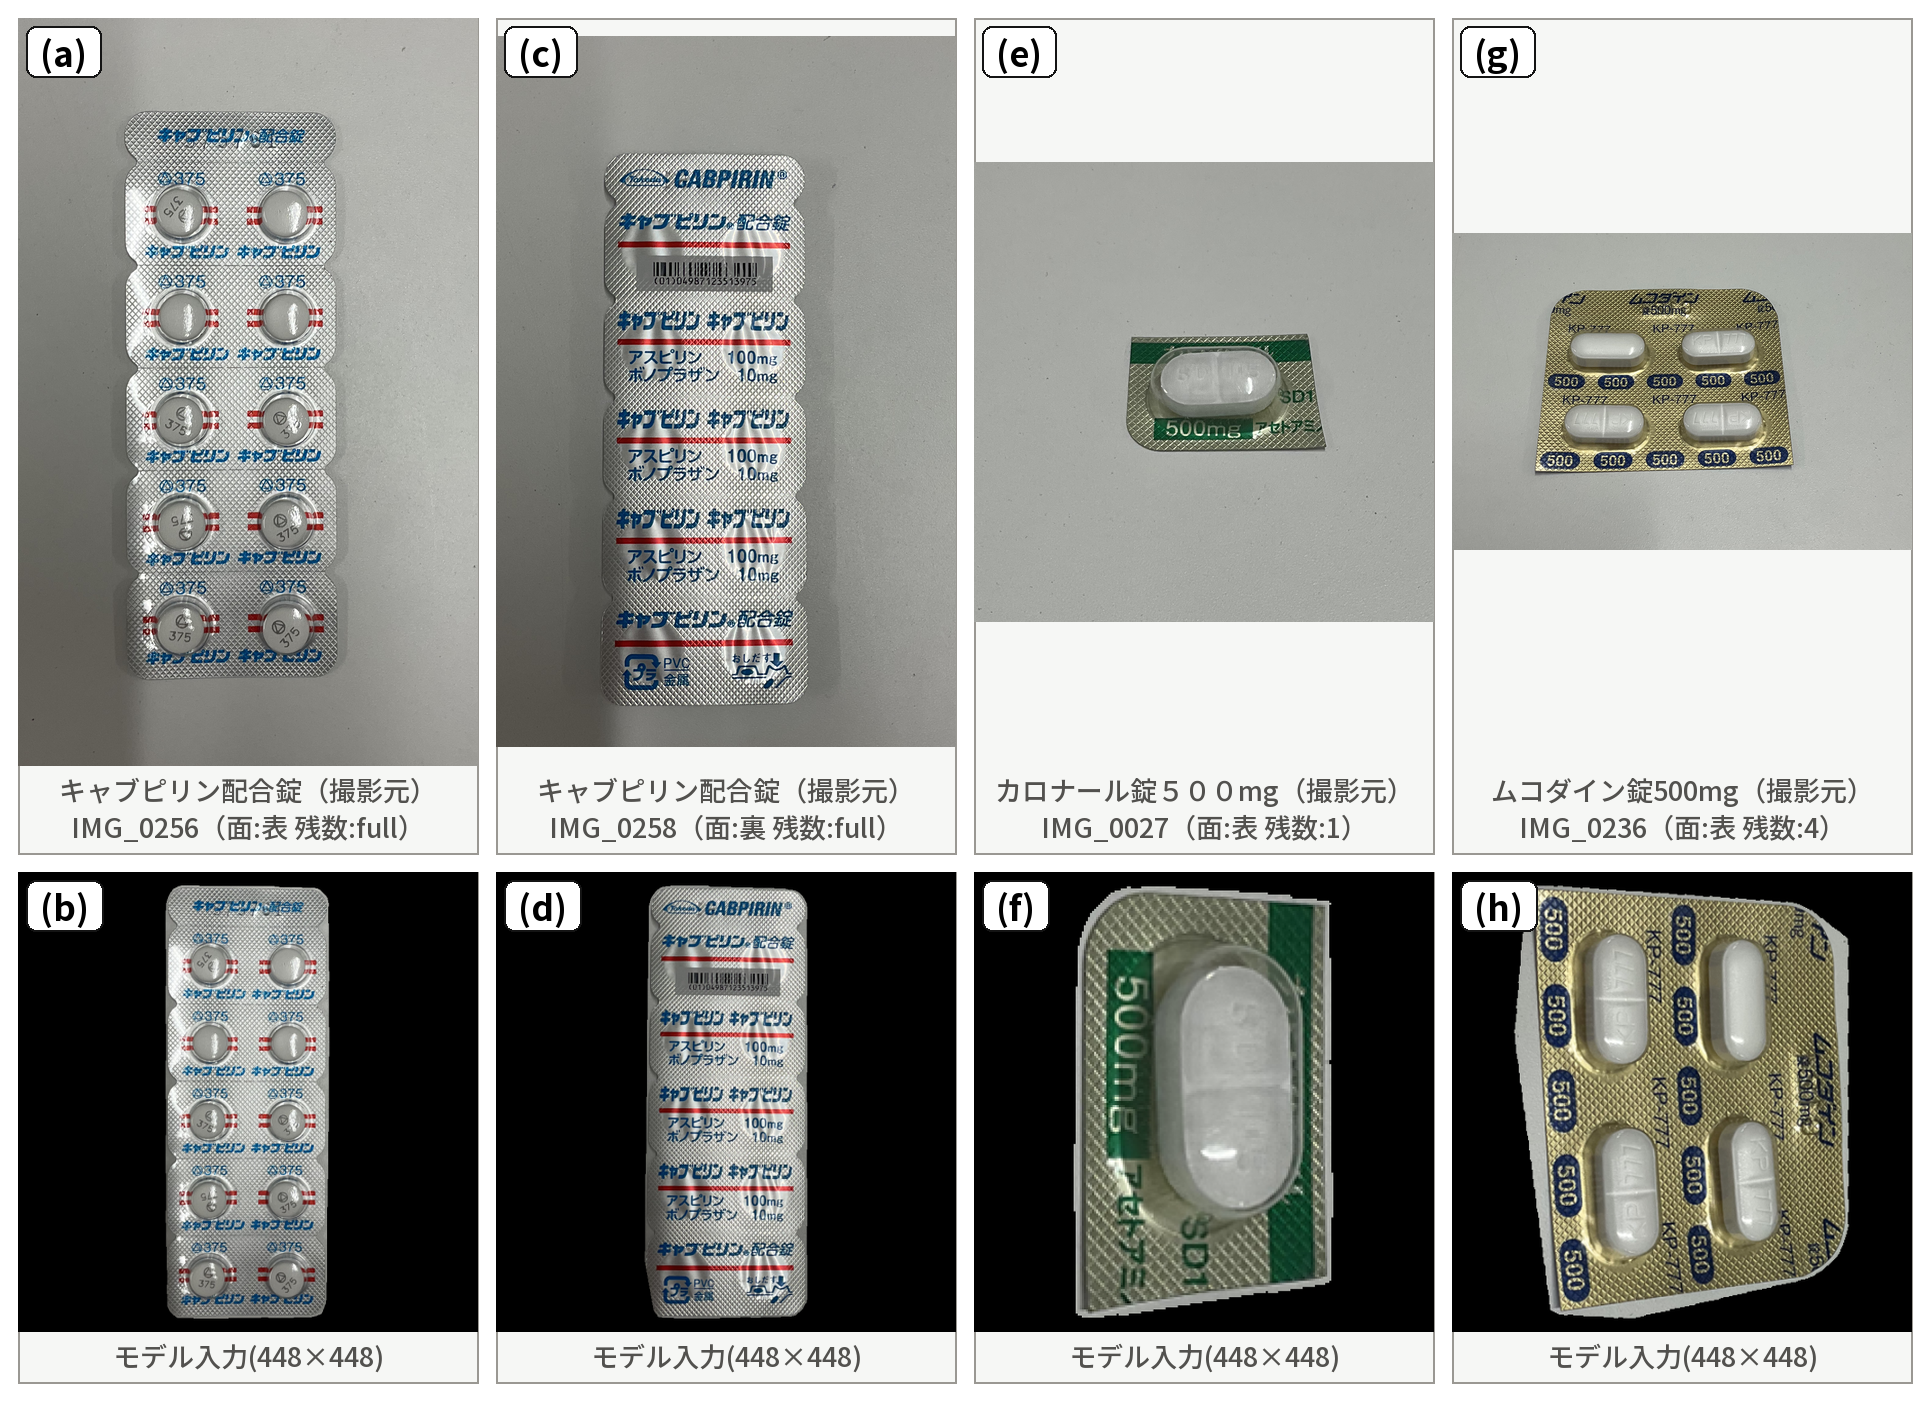
\includegraphics[width=\linewidth]{figures/generated/internal_eval_examples.png}
  \caption[薬剤部で撮影した評価画像の元画像とモデル入力]{薬剤部で撮影した評価画像の元画像と保存済みモデル入力の対応例．
  （a）（b）IMG\_0256（表面フルシート），
  （c）（d）IMG\_0258（裏面フルシート），
  （e）（f）IMG\_0027（表面・1錠），
  （g）（h）IMG\_0236（表面・4錠）である．
  各組の左が撮影元画像，右が背景除去・向き補正・448画素正方形化後のモデル入力である．
  画像は近畿大学病院薬剤部で撮影され，著者が保存済み評価データから再配置した．}
  \label{fig:internal_eval_examples}
\end{figure}

図\ref{fig:internal_eval_examples}では，元画像内の包装占有率や向きが異なっても，
モデル入力では包装が黒背景の448画素正方形へ正規化されることを確認できる．
撮影元287枚はすべてPNG形式・3024$\times$4032画素であった．
一方，EXIFの撮影日時，端末メーカーおよび端末型番は287枚すべてで欠落していた．
したがって，撮影端末，距離，照明，撮影セッションを画像の記録から復元できなかった．

文字列$s$にNFKC正規化と小文字化を適用する．
続いて，空白，読点，句点，中点，コロン，ハイフン，アンダースコア，スラッシュ，バックスラッシュ，丸括弧，角括弧，かぎ括弧，二重かぎ括弧を除去する．
この関数を$g(s)$とする．
保存済み評価実装の一致判定$M(a,b)$は，$g(a)=g(b)$，または$g(a)$が$g(b)$の部分文字列である場合に真となる．
画像$x_i$に対するモデルのTop-1出力を$\hat{y}_i$，記録済み正解ラベルを$y_i$とする．
Top-1精度は式\eqref{eq:top1}で求める．

\begin{equation}
  \operatorname{Accuracy}
  =
  \frac{1}{n}
  \sum_{i=1}^{n}
  \mathbf{1}\!\left(M(y_i,\hat{y}_i)\right)
  \label{eq:top1}
\end{equation}

この実装は正規化後の完全一致より緩い．
このため本報告書では，実装規則を開示したうえで，保存済み予測を$g(y_i)=g(\hat{y}_i)$の完全一致でも再集計し，両判定の正解数を比較する．
再集計の結果は\ref{sec:data_audit_results}節に示す．
Wilson区間，マクロ平均およびブートストラップ区間は，両判定の正解数が一致することを確認したうえで，保存済み判定に基づく集計値として示す．

クラス間の枚数の偏りを考慮するため，クラス別正解率のマクロ平均も式\eqref{eq:macro}で求める．
ここで$D$はクラス集合，$n_d$はクラス$d$の画像数である．

\begin{equation}
  \operatorname{MacroAccuracy}
  =
  \frac{1}{|D|}
  \sum_{d \in D}
  \frac{1}{n_d}
  \sum_{i : y_i = d}
  \mathbf{1}\!\left(M(y_i,\hat{y}_i)\right)
  \label{eq:macro}
\end{equation}

保存済み予測の薬剤別不確実性を補足するため，41クラスをクラスタとして復元抽出するブートストラップも用いる．
各反復では41クラスを復元抽出し，抽出したクラス別正解率の平均を求める．
乱数シードを260727に固定して10,000回反復し，2.5および97.5パーセンタイルを薬剤をクラスタとするブートストラップ95\%区間とする．
これは41クラスの分布に対する記述的な区間であり，新しい薬剤への一般化を示す区間ではない．

二項比率の95\%信頼区間にはWilson区間を用いる．
観測比率を$\hat{p}$，標本数を$n$，$z=1.96$とすると，区間は式\eqref{eq:wilson}で表す．

\begin{equation}
  \mathrm{CI}_{95\%}
  =
  \frac{
    \hat{p}+\frac{z^2}{2n}
    \pm
    z\sqrt{\frac{\hat{p}(1-\hat{p})}{n}+\frac{z^2}{4n^2}}
  }{
    1+\frac{z^2}{n}
  }
  \label{eq:wilson}
\end{equation}

同じ画像に対する2方式の正誤を比較する場合は，対応のある二値データとしてMcNemar検定を用いる．
方式Aのみが正解した画像数を$b$，方式Bのみが正解した画像数を$c$とする．
帰無仮説の下で不一致対の各方向は確率$1/2$で生じるため，両側の正確$p$値は式\eqref{eq:mcnemar_exact}で求める．

\begin{equation}
  p_{\mathrm{exact}}
  =
  \min\!\left\{
    1,\,
    2\sum_{k=0}^{\min(b,c)}
    \binom{b+c}{k}
    \left(\frac{1}{2}\right)^{b+c}
  \right\}
  \label{eq:mcnemar_exact}
\end{equation}

本研究では両側$p<0.05$を有意差の基準とする．
ただし，有意差が認められない結果は，2方式の統計的同等性を示すものではない．
不一致対がない場合，すなわち$b+c=0$の場合も，式\eqref{eq:mcnemar_exact}の正確両側$p$値は1となる．
正確McNemar検定は，各画像対の不一致方向が画像対間で独立であることを仮定する．
本評価集合には同じクラスに属する複数画像が含まれ，独立した撮影セッションを識別する情報も保存されていない．
したがって，この独立性は確認できなかった．
本報告書の$p$値は保存済み287画像内の探索的な記述値として示し，薬剤または撮影条件の母集団に対する確認的推論には用いない．

\subsubsection{追加学習していないQwen3.5-4Bとの比較}

追加学習前の基準として，LoRAを適用していないQwen3.5-4Bの保存済み予測287件を再集計する．
この実行では素画像を入力し，プロンプトは
「この錠剤は何という薬ですか？薬剤名だけで答えてください．」である．
保存時の判定は，正規化した正解薬剤名が生成文に含まれる場合を成功としていた．
本報告書ではこれを再現するとともに，式\eqref{eq:top1}より厳しい
$g(y_i)=g(\hat{y}_i)$の完全一致でも再集計する．
3系列の予測は，薬剤名と画像ファイル名を結合した識別子で単剤マニフェストへ結合し，287件すべてを一意に対応させる．

追加学習していない側とLoRAを適用した側では，入力の前処理，入力画像サイズ，実行環境および出力の制御が異なる．
したがって，これは保存済みの実行同士の比較であり，LoRAの有無だけを変えた比較ではない．

\subsubsection{外部サービスとの対応比較}

外部サービスとの比較には，2026年6月24日に保存したモデル文字列\texttt{gemini-3.5-flash}の予測を用いる\cite{google_gemini35flash}．
Gemini側では元画像を最大589,824画素へ縮小し，JPEG品質90へ変換する．
プロンプトには，学習対象と同じ41クラスの候補一覧を与える．
Geminiとver6は，薬剤名と画像ファイル名を結合した識別子で対応付ける．
さらに，元画像と正解ラベルの一致を確認する．
正誤は保存済み予測と正解ラベルの完全一致で再集計する．
モデルリビジョン，温度，乱数シードが記録されていないため，APIへ再問い合わせせず，保存済みCSVを一次資料とする．

本評価では5分割交差検証を用いない．
学習元は薬剤ごとに1組の収集画像であり，評価対象は薬剤部で撮影した評価画像である．
派生画像だけを分割すると，同一の収集元画像に由来する画像が学習用分割と検証用分割に混入する．
また，評価画像だけを5分割してもモデルを再学習しないため，同じ予測を分割集計するだけになる．
各薬剤について5組以上の独立した収集元画像がないため，元画像単位のグループ化交差検証を構成できなかった．
このため，全287枚の点推定を主な集計値とし，Wilson区間は画像単位の独立性を仮定した参考値として併記する．

\subsubsection{合成複数薬剤画像}\label{sec:multi_eval}

複数薬剤評価には，元写真を黒い隙間で区切り，薬剤数が2，3，5，8の合成複数薬剤画像を各100枚用いる．
この合成複数薬剤画像400枚は，収集画像学習ver1からver9まで共通である．
ただし，ver1からver3は評価時に領域を検出し，ver4以降は同じ400枚から生成した固定評価キャッシュの1,800領域を用いる．
画像中の連結領域を検出し，各領域を単剤モデルへ入力する．
領域分割では，画素の最大RGB値が18を超える領域を前景とし，$7\times7$の形態学的クロージングを2回適用した後，外側輪郭を抽出する．
さらに，画像全体に対する外接矩形の面積比が2.5\%以上で，短辺が100画素以上の領域だけを識別対象とする．
したがって，この領域分割は，薬剤間に黒い隙間があり，包装同士が接触しない配置を前提とする連結領域分割であり，一般的な物体検出器ではない．
画像$i$について，保存順の正解薬剤ラベル列を$Y_i$，予測ラベル列を$\hat{Y}_i$とする．
保存済み実装では，$\hat{Y}_i$の予測を順に調べ，一致判定$M$が真となる未対応の正解ラベルのうち先頭の要素へ貪欲に一対一対応付けする．
対応できた個数を$c_i^{\mathrm{greedy}}$とする．
部分文字列一致を許す$M$では，この個数は一般に保存順へ依存し得る．
合成複数薬剤画像の総数を$N_{\mathrm{multi}}$とする．
画像単位完全一致率は式\eqref{eq:exact_match}で求める．

\begin{equation}
  \operatorname{ExactMatch}
  =
  \frac{1}{N_{\mathrm{multi}}}
  \sum_{i=1}^{N_{\mathrm{multi}}}
  \mathbf{1}\!\left(c_i^{\mathrm{greedy}}=|Y_i|=|\hat{Y}_i|\right)
  \label{eq:exact_match}
\end{equation}

領域ラベル一致率は式\eqref{eq:region_acc}で求める．

\begin{equation}
  \operatorname{RegionLabelMatch}
  =
  \frac{\sum_{i=1}^{N_{\mathrm{multi}}}c_i^{\mathrm{greedy}}}
       {\sum_{i=1}^{N_{\mathrm{multi}}}|Y_i|}
  \label{eq:region_acc}
\end{equation}

この指標は正解ラベルに対する対応率であり，過検出を分母へ含めない．
過検出は，画像単位完全一致率と検出領域数によって別途評価する．
また，本指標は画像内ラベル列を保存順に貪欲対応した一致数であり，検出領域の物理的位置ごとの正誤率ではない．
保存済み予測を正規化後の厳密一致で再集計すると対応候補は同一ラベルだけとなり，保存順への依存はなくなる．
このため，合成複数薬剤の集計についても厳密一致で再集計し，保存済み集計値と比較する．
再集計の結果は\ref{sec:data_audit_results}節に示す．
これらの評価画像は合成複数薬剤画像であり，薬剤同士の重なりや実背景を含まない．
したがって，実画像における複数薬剤識別性能とは区別する．
図\ref{fig:eval_inputs}に評価入力の例を示す．

\begin{figure}[H]
  \centering
  \begin{tikzpicture}[
    frame/.style={draw,minimum height=4.1cm,align=center},
    package/.style={draw,rounded corners=1mm,fill=white,minimum width=1.4cm,minimum height=2.6cm,font=\scriptsize,align=center}
  ]
    \node[frame, minimum width=4.6cm, fill=black!8] (single) {};
    \node[package] at (single.center) {PTP包装\\1点};
    \node[font=\small, below=1mm of single] {単剤評価入力};

    \node[frame, minimum width=7.8cm, fill=black!85, right=1.0cm of single] (multi) {};
    \node[package] at ([xshift=-1.8cm]multi.center) {PTP包装\\1点};
    \node[package] at ([xshift=1.8cm]multi.center) {PTP包装\\1点};
    \node[font=\small, below=1mm of multi] {黒い間隔を設けた合成複数薬剤入力};
  \end{tikzpicture}
  \caption{評価入力の構成を示す模式図（左：単剤，右：合成複数薬剤）}
  \label{fig:eval_inputs}
\end{figure}

\begin{figure}[H]
  \centering
  \includegraphics[width=\linewidth]{figures/generated/multi_actual_examples.png}
  \caption[固定400枚に含まれる合成複数薬剤画像の実例]{固定400枚に含まれる合成複数薬剤画像の実例．
  （a）2薬剤，ID 2薬剤\_0001，（b）5薬剤，ID 5薬剤\_0001，
  （c）8薬剤，ID 8薬剤\_0001である．
  評価用の単剤実写真を黒い隙間で区切って合成した画像であり，
  実写の複数薬剤配置ではない．包装同士の接触，重なり，複雑な背景を含まない．
  著者が保存済み評価画像を再配置した．}
  \label{fig:multi_actual_examples}
\end{figure}

図\ref{fig:multi_actual_examples}に，模式図\ref{fig:eval_inputs}に対応する実際の入力を示す．

\subsubsection{信頼ゲート}

条件Cのモデルへ，信頼できない入力に対する回答を保留する信頼ゲートを適用する．
これは探索的追試ver6とは異なるアダプタに対する予備評価であり，ver6では信頼ゲートを評価していない．
既知薬剤には薬剤部で撮影した評価画像287枚を用い，保存済み記録ラベル単位で校正集合139枚と最終評価集合148枚に事前分割する．
未知薬剤には，学習対象の41件の保存済み記録ラベルに含まれない薬剤の収集画像125枚を用い，薬剤ラベル単位で校正集合67枚と最終評価集合58枚に事前分割する．
既知薬剤と未知薬剤のいずれも，校正集合と最終評価集合の薬剤ラベルに重複はなかった．
全評価画像について，学習画像と同一の画像が含まれていないことを確認する．
ただし，この確認は，再圧縮や切り出しを経た近い画像が混入していないことまでは保証しない．

信頼ゲート専用の正規化関数$h(s)$は，まず大文字と小文字を区別せずに\texttt{<think>...</think>}区間を除去する．
次に，Unicode NFKCを適用し，前後の空白を除去して小文字化する．
先頭が「薬剤名は」「これは」「回答は」のいずれかであれば，該当する接頭句を1つだけ除去する．
末尾が「です」「になります」のいずれかであれば，該当する接尾句を1つだけ除去する．
最後に，空白と保存実装で列挙した句読点・区切り記号を除去する．
学習対象の保存済み記録ラベル集合を$W_{\mathrm{raw}}$とし，信頼ゲートで照合する既知集合を$W=\{h(w)\mid w\in W_{\mathrm{raw}}\}$とする．

Top-3ビーム探索で得た候補を系列スコアの降順に並べ，$s_1 \geq s_2 \geq s_3$とする．
$s_k$は，第$k$候補について生成処理が返す長さ調整済み系列スコアである．
$s_k$は反復ペナルティを含む生成設定に依存するため，モデル固有の校正済み確率とは扱わない．
候補間マージン$m$を式\eqref{eq:margin}で定義する．

\begin{equation}
  m = s_1 - s_2
  \label{eq:margin}
\end{equation}

11視点のTTA出力を$\hat{y}^{(1)},\ldots,\hat{y}^{(11)}$，各出力の信頼ゲート専用正規化結果を$\tilde{y}^{(j)}=h(\hat{y}^{(j)})$とする．
正規化後の最頻値を$v$とすると，TTA多数決一致率$a$は式\eqref{eq:tta_agree}で表す．
同数首位がある場合は，保存実装に従い，11視点の列で最初に現れた候補の正規化値を$v$とする．

\begin{equation}
  a = \frac{1}{11}\sum_{j=1}^{11}\mathbf{1}\!\left(\tilde{y}^{(j)} = v\right)
  \label{eq:tta_agree}
\end{equation}

信頼ゲートは3段階で構成する．
第1段階では，モデル出力へ$h$を適用し，既知集合$W$との厳密一致を確認する．
第2段階では，元画像，回転，左右反転，明度，コントラスト，ノイズからなる11視点のテスト時拡張（Test-Time Augmentation：TTA）を用いる．
多数決結果が既知薬剤名であることを確認する．
さらに，多数決結果がTop-1予測と一致し，一致率がしきい値以上であることを確認する．
第3段階では，Top-3ビーム探索の第1候補系列スコア$s_1$と候補間マージン$m$をしきい値と比較する．
アルゴリズム\ref{alg:trust_gate}に判定順序を示す．

\begin{algorithm}[H]
  \caption{信頼ゲートによる回答と保留の判定}
  \label{alg:trust_gate}
  \small
  \begin{algorithmic}[1]
    \REQUIRE 画像$x$，学習済みモデル$f_\theta$，正規化関数$h$，既知集合$W$，しきい値$\tau_s$，$\tau_m$，$\tau_a$
    \ENSURE $h$で正規化したクラス名または保留
    \STATE $f_\theta$のTop-3ビーム探索により候補$\hat{y}_1,\hat{y}_2,\hat{y}_3$と$s_1 \geq s_2 \geq s_3$の系列スコアを得る
    \STATE $\tilde{y}_1 \gets h(\hat{y}_1)$
    \IF{$\tilde{y}_1 \notin W$}
      \RETURN 保留
    \ENDIF
    \STATE 11視点のTTA出力へ$h$を適用し，多数決$v$と一致率$a$を求める
    \IF{$v \notin W$，または$v \neq \tilde{y}_1$，または$a < \tau_a$}
      \RETURN 保留
    \ENDIF
    \IF{$s_1 < \tau_s$，または$s_1 - s_2 < \tau_m$}
      \RETURN 保留
    \ENDIF
    \RETURN $\tilde{y}_1$
  \end{algorithmic}
\end{algorithm}

\enlargethispage{2\baselineskip}
回答するには，既知薬剤名集合への所属，Top-1とTTA多数決の一致，TTA一致率，系列スコア，候補間マージンの全条件を満たす必要がある．
いずれか1条件でも満たさない場合は，アルゴリズム\ref{alg:trust_gate}の順序で保留する．
しきい値は校正集合だけで決定し，最終評価集合の推論前に固定する．
未知薬剤に対して既知薬剤名を回答することを，以下では危険通過と呼ぶ．
既知薬剤の誤回答を0件，未知薬剤の危険通過を67枚中3枚以下とする制約下で，既知薬剤への正しい回答数を最大化する．
固定後は最終評価集合の結果を見て変更しない．
指標には，既知薬剤への回答率，回答した既知薬剤の正解率，未知薬剤の保留率を用い，各比率にWilson法による95\%信頼区間を付す．
なお，信頼ゲートでは信頼信号を得るためTop-3ビーム探索を用いるため，単剤評価の貪欲法による生成とは生成方法が異なる．

%----------------------------------------------------------------------
\clearpage
\section{実験結果・考察}\label{sec:results}
%----------------------------------------------------------------------

\subsection{実験環境とデータ監査結果}

\subsubsection{実験環境と撮影記録}

主条件Dと探索的ver6の実験環境を表\ref{tab:environment}に示した．
両条件の学習にはNVIDIA H100を1台使用した．
モデルリビジョンを固定し，実行時のPythonおよび主要ライブラリの版を記録した．
乱数シードは42としたが，速度を優先してCUDAの決定論的アルゴリズムを無効にした．
このため，ビット単位で同一の再現は保証されなかった．
本研究は人を対象とする実験ではなく，被験者を用いず，PTP包装画像を評価対象とした．
評価画像はPTP包装だけを写した画像であり，患者を識別できる情報は含まれていなかった．

\begin{table}[H]
  \centering
  \caption{主条件Dおよび探索的ver6の実験環境}
  \label{tab:environment}
  \small
  \setlength{\tabcolsep}{3pt}
  \begin{tabular}{|>{\raggedright\arraybackslash}p{3.0cm}|>{\raggedright\arraybackslash}p{4.7cm}|>{\raggedright\arraybackslash}p{4.7cm}|}
    \hline
    項目 & 主条件D & 探索的ver6 \\ \hline
    GPU & NVIDIA H100，VRAM 93.096 GiB，1台 & 同左 \\ \hline
    OS／Python & Linux 6.8.0，glibc 2.39／Python 3.13.5 & 同左 \\ \hline
    主要ライブラリ & PyTorch 2.11.0，CUDA 12.8，cuDNN 9.19，Transformers 5.14.1，PEFT 0.19.1 & 同左 \\ \hline
    基盤モデル & \multicolumn{2}{p{9.7cm}|}{\shortstack[l]{Qwen/Qwen3.5-4B，リビジョン\\
    \texttt{851bf6e806efd8d0a36b}\\
    \texttt{00ddf55e13ccb7b8cd0a}}} \\ \hline
    LoRA & ランク16，係数32，BF16 & ランク32，係数64，BF16 \\ \hline
    学習対象層 & q，k，v，o射影およびgate，up，down射影 & 同左 \\ \hline
    学習可能パラメータ数 & 21,233,664 & 42,467,328 \\ \hline
    画像拡張 & 撮影変動対応17条件 & 条件Cと同じ回転12条件＋明度5条件 \\ \hline
    バッチ & マイクロバッチ16，勾配累積8，実効バッチ128 & 同左 \\ \hline
    エポック数／乱数シード & 5／42 & 5／42 \\ \hline
  \end{tabular}
\end{table}

薬剤部で撮影した評価画像の撮影条件として確認できた事項を表\ref{tab:capture_conditions}に示した．
端末，距離，角度，照明および背景の値は保存記録から確認できなかったため，推測で補わなかった．

\begin{table}[H]
  \centering
  \caption{薬剤部で撮影した評価画像の撮影・前処理記録}
  \label{tab:capture_conditions}
  \small
  \begin{tabular}{|p{4.0cm}|p{8.2cm}|}
    \hline
    項目 & 確認結果 \\ \hline
    撮影場所 & 近畿大学病院薬剤部 \\ \hline
    撮影日 & 元画像ディレクトリ名は2026年4月9日撮影を示したが，PNG内に独立した撮影日時を確認できなかった． \\ \hline
    撮影端末・セッション数 & PNG内に機種情報がなく，撮影セッションIDも保存されていなかった． \\ \hline
    元画像解像度 & 評価マニフェスト287枚はすべて3,024 $\times$ 4,032画素であった． \\ \hline
    距離・角度・照明・背景 & 数値または条件を記録していなかった． \\ \hline
    表裏の記録 & 保存台帳と評価マニフェストに表裏を記録し，表212枚，裏75枚であった． \\ \hline
    フル／部分シート & フルシート29枚，1錠から9錠の部分シート258枚であった． \\ \hline
    背景除去 & 色しきい値と形態学的処理で前景マスクを作成し，外側輪郭の凸包を透視変換した後，448 $\times$ 448画素の黒背景へ配置した． \\ \hline
  \end{tabular}
\end{table}

図\ref{fig:loss_curve}にver6の学習損失を示した．
最終ログに記録された学習損失は$2.8 \times 10^{-5}$であった．
4エポック以降はおおむね$1 \times 10^{-5}$台で推移したが，最終ログ点は直前の区間より高い値であった．
条件Cの最終損失は$1.3 \times 10^{-5}$であったが，学習損失の大小だけで評価精度を比較できなかった．
独立した検証集合の損失を測定していないため，過学習の有無および5エポックが最適であったかは判断できなかった．

\begin{figure}[H]
  \centering
  \begin{tikzpicture}
    \begin{axis}[
      width=13.2cm,
      height=6.0cm,
      ymode=log,
      xlabel={エポック},
      ylabel={学習損失},
      xmin=0, xmax=5,
      tick label style={font=\small},
      label style={font=\small},
      grid=major
    ]
      \addplot[blue,thick,mark=none] coordinates {
        (0.0074,3.130116) (0.1339,0.177026) (0.2604,0.044856) (0.3943,0.020968) (0.5208,0.009653) (0.6473,0.008702) (0.7738,0.001153) (0.9077,0.00808)
        (1.0342,0.000574) (1.1607,0.000243) (1.2871,0.00022) (1.4211,0.000153) (1.5475,0.000107) (1.674,0.000144) (1.8005,0.00033) (1.927,0.000237)
        (2.0609,8.7e-05) (2.1874,0.000144) (2.3139,5.1e-05) (2.4404,0.000131) (2.5743,0.00038) (2.7008,4.3e-05) (2.8272,3.1e-05) (2.9537,3e-05)
        (3.0877,2.8e-05) (3.2141,2.3e-05) (3.3406,1.7e-05) (3.4671,1.9e-05) (3.5936,1.9e-05) (3.7275,1.9e-05) (3.854,1.4e-05) (3.9805,1.6e-05)
        (4.107,1.4e-05) (4.2409,1.6e-05) (4.3674,1e-05) (4.4938,1.1e-05) (4.6203,1.3e-05) (4.7542,1e-05) (4.8807,1.1e-05) (5.0,2.8e-05)
      };
    \end{axis}
  \end{tikzpicture}
  \caption{ver6の学習損失（縦軸は対数目盛）}
  \label{fig:loss_curve}
\end{figure}

\subsubsection{データおよび監査結果}\label{sec:data_audit_results}

\ref{sec:provenance_audit}節の手順による収集画像の由来監査の結果は，次のとおりであった．
収集画像は41クラス・42ファイルであった．
32ファイルは現行の収集記録と直接照合できた．
残る10ファイルは，削除前の収集記録から出典記録または出典候補を確認した．
一方，この10ファイルについては，元画像から現存画像までの加工の履歴をたどれなかった．
また，収集画像と薬剤部で撮影した評価画像287枚に同一の画像は含まれていなかった．

\ref{sec:single_eval}節および\ref{sec:multi_eval}節の判定規則に関する再集計の結果は，次のとおりであった．
保存済み予測を正規化後の完全一致で再集計しても，単剤の正解数はver4条件D，条件C，ver6，ver7でそれぞれ280，283，286，284であり，保存済み集計値と変わらなかった．
合成複数薬剤画像でも，画像単位完全一致はそれぞれ331，356，374，380，領域ラベル一致数はそれぞれ1,725，1,752，1,773，1,780であり，保存済み集計値と変わらなかった．
両判定の正解数が一致したため，以降のWilson区間，マクロ平均およびブートストラップ区間は保存済み判定に基づく集計値として示した．

\subsection{初期実画像方式と収集画像学習への移行}

研究初期には，近畿大学病院薬剤部で撮影した41クラスに属する287枚を学習元と評価用に分ける方式を用いた．
乱数シード42で元画像単位に分割し，213枚を学習用，74枚を評価用とした．
学習用画像へ11提示条件の拡張を適用し，Qwen3.5-4BをLoRAで追加学習した．
拡張していない評価用元画像74枚では，74枚すべてが正解であった．
同じ74枚から生成した回転・明度変化を含む814枚では799/814枚，98.2\%であった．
後者の814枚は独立して撮影した814枚ではなく，74枚から生成した派生画像であった．

単一分割への依存を確認するため，同じ287枚を元画像単位で5分割し，各分割を1回ずつ評価用とする交差検証も行った．
分割別のTop-1精度は，58/58枚，58/58枚，56/57枚，55/57枚，56/57枚であり，順に100.0\%，100.0\%，98.2\%，96.5\%，98.2\%であった．
全分割を統合すると283/287枚，98.6\%であった．
分割別精度の平均と標準偏差は98.6\%$\pm$1.5\%であった．
これは初期実画像方式の内部検証であり，後述する収集画像学習モデルの外部評価ではなかった．

実画像を学習元とする方式について，1薬剤当たりの学習元画像数も比較した．
6枚以上の元画像を持つ33薬剤を対象とし，同じ79枚を評価した結果を表\ref{tab:fewshot_history}に示した．

\begin{table}[H]
  \centering
  \caption{初期実画像方式における1薬剤当たりの学習元画像数とTop-1精度（対象33薬剤，固定評価79枚）}
  \label{tab:fewshot_history}
  \small
  \begin{tabular}{|c|r|r|}
    \hline
    1薬剤当たりの学習元画像数 & 拡張後の学習画像数 & Top-1精度 \\ \hline
    1 & 363 & 67.1\% \\ \hline
    2 & 726 & 87.3\% \\ \hline
    4 & 1,452 & 91.1\% \\ \hline
    利用可能な全画像（5--8枚） & 1,947 & 98.7\% \\ \hline
  \end{tabular}
\end{table}

同一の33薬剤と固定評価79枚を用いた比較では，学習元画像数の増加に伴って精度が上昇した．
ただし，乱数シード42による1回の比較であり，薬剤ごとの画像数にも差があるため，必要撮影枚数を確定する結果ではなかった．
薬剤を追加するたびに，複数の学習用実画像を撮影して整理する必要があった．
この撮影・整理負担が，対象薬剤数を増やすうえでの課題となった．

また，学習元213枚と評価用元画像74枚を固定し，1元画像当たりの提示条件数だけを変えた結果を表\ref{tab:augmentation_history}に示した．

\begin{table}[H]
  \centering
  \caption{初期実画像方式における提示条件数とTop-1精度（学習元213枚，固定評価74枚）}
  \label{tab:augmentation_history}
  \small
  \begin{tabular}{|c|r|r|}
    \hline
    提示条件数 & 学習画像数 & Top-1精度（正解数/74） \\ \hline
    1 & 213 & 73.0\%（54/74） \\ \hline
    3 & 639 & 87.8\%（65/74） \\ \hline
    5 & 1,065 & 90.5\%（67/74） \\ \hline
    7 & 1,491 & 95.9\%（71/74） \\ \hline
    11 & 2,343 & 97.3\%（72/74） \\ \hline
    17 & 3,621 & 100.0\%（74/74） \\ \hline
  \end{tabular}
\end{table}

この単一分割では提示条件数の増加に伴って観測精度が上昇した．
一方，各提示条件数での実験は1回だけであり，評価枚数も74枚であった．
また，17提示条件には同一画素となる0度回転と明度倍率1.0が含まれる．
したがって，17提示条件が一般に最適であることや，精度差が提示条件数だけに起因することは示さなかった．

以上から，少数の元画像から複数の見え方を生成する方針を維持しつつ，残存錠数や切り出し範囲を変えた学習用写真を個別に撮影せずに済む構成とするため，フルシート表裏の収集画像を学習元とする方式へ移行した．

\subsection{収集画像学習ver1からver3}

実験管理上の保存名は「Web画像学習」であるが，本報告書では出典監査の完了状況を考慮し，一般名称として「収集画像学習」を用いる．
収集画像学習ver1からver3では，同じ評価画像287枚と合成複数薬剤画像400枚を用いながら，基画像の構成を段階的に変更した．
結果を表\ref{tab:web_v1_v3}に示した．

\begin{table}[H]
  \centering
  \caption{収集画像学習ver1からver3の入力と評価結果}
  \label{tab:web_v1_v3}
  \scriptsize
  \setlength{\tabcolsep}{2pt}
  \begin{tabular}{|c|r|r|c|c|p{2.7cm}|r|r|}
    \hline
    実験 & 基画像数 & \shortstack{17種類\\提示後} & 量子化 & LoRA & GPU／実効バッチ & 単剤Top-1 & \shortstack{画像単位\\完全一致} \\ \hline
    ver1 & 457 & 7,769 & 4ビット & r8，q/v & RTX 4070 Ti SUPER／16 & 259/287（90.24\%） & 245/400（61.25\%） \\ \hline
    ver2 & 451 & 7,667 & 4ビット & r8，q/v & RTX 4070 Ti SUPER／16 & 255/287（88.85\%） & 252/400（63.00\%） \\ \hline
    ver3 & 1,265 & 21,505 & 4ビット & r8，q/v & H100／128 & 281/287（97.91\%） & 371/400（92.75\%） \\ \hline
  \end{tabular}
\end{table}

ver1では，RTI 41枚と1錠区画416枚を基画像とし，4ビットQLoRAで学習した．
評価画像287枚は学習に用いておらず，その287枚に対する単剤Top-1精度は90.24\%であった．
この結果から，収集画像を学習元とする方針には一定の見込みがあると考えた．
一方，初期実画像方式より精度が低く，部分画像の空間的多様性が課題として残った．

ver2では，各薬剤についてRTIを1枚生成した．
さらに，面別にフルシートを各1枚，1錠区画を各2枚，上半分を各1枚，上1／4区画を各1枚生成し，式\eqref{eq:base_count_v2}の合計11枚とした．

\begin{equation}
  N^{\mathrm{ver2}}_d = 1 + 2(1 + 2 + 1 + 1) = 11
  \label{eq:base_count_v2}
\end{equation}

1錠区画画像は同じ位置を重複して用いており，包装内の異なる位置を網羅していなかった．
ver1から単剤Top-1は1.39パーセントポイント低下し，画像単位完全一致率は1.75パーセントポイント上昇した．
ただし，基画像の構成も異なるため，一つの変更だけの効果とは解釈しなかった．

ver3では，異なる錠剤セル，縦2分割画像，縦4分割画像を加え，通常の薬剤については基画像を31枚生成した．
基画像数は1,265枚，17種類の提示条件適用後は21,505枚であり，単剤Top-1は97.91\%へ上昇した．
ただし，ver2からver3では基画像構成，画像枚数，使用GPU，実効バッチが同時に変化した．
したがって，改善を部分画像の位置追加だけに帰属できなかった．
また，同じ287枚をver1以降の条件検討に反復使用したため，ver1からver3の評価はいずれも内部開発評価であった．

\subsection{収集画像学習ver4（条件AからDの比較）}\label{sec:ver4_conditions}

表\ref{tab:conditions}に条件AからDの設定と結果を示した．
評価画像，エポック数，乱数シードは全条件で共通とした．
条件Aはver3の設定を基準として4ビットQLoRAを再構成した条件であるが，ver3本番実行の再現結果とは扱わない．
条件Aはver3と同じ基画像1,265枚，同じ17提示条件，同じ4ビット量子化を用いたが，単剤Top-1はver3の97.91\%に対して94.77\%であった．
ver3と条件Aでは，同一条件を意図しても実行環境と実装が完全には一致しなかった．
したがって，条件Aはver3の再現結果ではなく，条件BからDと比較するための基準として用いた．
条件Bでは量子化を行わなかったほか，勾配チェックポイントとマイクロバッチ構成も変更した．
条件CはLoRAのランク，スケーリング係数，対象層を同時に増やした．
条件Dは条件Cの画像拡張を撮影変動対応の重複しない17条件へ置き換えた．
手元の設計資料では条件Dが主条件とされていたが，第三者が検証できる形で事前に登録した条件ではなかった．
このため，本報告書では条件Dを主結果として扱いつつ，事前登録済みの条件とは扱わなかった．

\begin{table}[H]
  \centering
  \caption{条件AからDの設定と評価結果}
  \label{tab:conditions}
  \scriptsize
  \begin{tabular}{|c|p{4.9cm}|r|r|r|}
    \hline
    条件 & 主な設定 & 単剤Top-1 & \shortstack{画像単位\\完全一致} & \shortstack{領域ラベル\\一致} \\ \hline
    A & 4ビットQLoRA，ランク8・係数16，q/v射影，ver3の17提示条件 & 272/287（94.77\%） & 307/400（76.75\%） & 1,696/1,800（94.22\%） \\ \hline
    B & BF16 LoRA，ランク8・係数16，q/v射影，ver3の17提示条件 & 276/287（96.17\%） & 320/400（80.00\%） & 1,714/1,800（95.22\%） \\ \hline
    C & BF16 LoRA，ランク16・係数32，q/k/v/o＋gate/up/down，ver3の17提示条件 & 283/287（98.61\%） & 356/400（89.00\%） & 1,752/1,800（97.33\%） \\ \hline
    D & BF16 LoRA，ランク16・係数32，q/k/v/o＋gate/up/down，撮影変動対応17提示条件 & 280/287（97.56\%） & 331/400（82.75\%） & 1,725/1,800（95.83\%） \\ \hline
  \end{tabular}
\end{table}

図\ref{fig:condition_comparison}に各条件の正解率を示した．
本報告書で主結果として扱う条件Dは，単剤Top-1が280/287（97.56\%），画像単位完全一致率が331/400（82.75\%），領域ラベル一致率が1,725/1,800（95.83\%）であった．
単剤Top-1のWilson法による95\%信頼区間は，画像単位の参考値として95.05\%から98.81\%であった．
保存済み予測から求めた薬剤別正解率のマクロ平均は96.82\%であり，薬剤をクラスタとするブートストラップ95\%区間は94.24\%から98.98\%であった．
薬剤別正解率の最低値は75.00\%であり，該当するクラスはタケキャブ錠20mg，ミヤBM錠，メトクロプラミド錠5mgであった．

保存済み予測を面，シート種別および残存錠数で層別に再集計した結果を表\ref{tab:condition_d_stratified}に示した．
再集計では新しい推論を行わず，条件Dの保存済み予測だけを入力とした．
保存時の判定と\ref{sec:single_eval}節の正規化後の厳密一致は287件すべてで一致し，層別の分母は面が表212枚・裏75枚，シート種別がフルシート29枚・部分シート258枚であった．

\begin{table}[H]
  \centering
  \caption{主条件Dの層別正解率（分母は評価画像287枚の内訳）}
  \label{tab:condition_d_stratified}
  \small
  \begin{tabular}{|l|l|r|r|}
    \hline
    層 & 区分 & 正解数／枚数 & 正解率 \\ \hline
    \multirow{2}{*}{面} & 表 & 205/212 & 96.70\% \\ \cline{2-4}
     & 裏 & 75/75 & 100.00\% \\ \hline
    \multirow{2}{*}{シート種別} & フルシート & 29/29 & 100.00\% \\ \cline{2-4}
     & 部分シート & 251/258 & 97.29\% \\ \hline
    \multirow{9}{*}{残存錠数} & 1錠 & 37/39 & 94.87\% \\ \cline{2-4}
     & 2錠 & 60/60 & 100.00\% \\ \cline{2-4}
     & 3錠 & 40/42 & 95.24\% \\ \cline{2-4}
     & 4錠 & 42/44 & 95.45\% \\ \cline{2-4}
     & 5錠 & 33/33 & 100.00\% \\ \cline{2-4}
     & 6錠 & 15/16 & 93.75\% \\ \cline{2-4}
     & 7錠 & 15/15 & 100.00\% \\ \cline{2-4}
     & 8錠 & 6/6 & 100.00\% \\ \cline{2-4}
     & 9錠 & 3/3 & 100.00\% \\ \hline
    全体 & 全画像 & 280/287 & 97.56\% \\ \hline
  \end{tabular}
\end{table}

裏面75枚とフルシート29枚は，いずれも誤分類が0件であった．
一方，表面は205/212枚であり，誤分類7件はすべて表面に生じた．
ただし，残存錠数別の分母は3枚から60枚までと偏りが大きく，錠数と正解率の関係を確定的に解釈できない．

\begin{table}[H]
  \centering
  \caption{主条件Dの誤分類7件（評価画像287枚）}
  \label{tab:condition_d_errors}
  \scriptsize
  \setlength{\tabcolsep}{2pt}
  \begin{tabular}{|p{1.5cm}|p{3.3cm}|p{3.6cm}|c|c|}
    \hline
    画像ID & 正解薬剤 & 条件Dの予測 & 面 & 錠数 \\ \hline
    IMG\_0020 & レバミピド錠100mg & プレドニン錠5mg & 表 & 1 \\ \hline
    IMG\_0027 & カロナール錠500mg & デエビゴ錠5mg & 表 & 1 \\ \hline
    IMG\_0039 & ミヤBM錠 & メチコバール錠500$\mu$g & 表 & 3 \\ \hline
    IMG\_0047 & タケキャブ錠20mg & ジャディアンス錠10mg & 表 & 3 \\ \hline
    IMG\_0079 & メトクロプラミド錠5mg & デエビゴ錠5mg & 表 & 4 \\ \hline
    IMG\_0236 & ムコダイン錠500mg & レボチロキシンNa錠50$\mu$g & 表 & 4 \\ \hline
    IMG\_0238 & ムコダイン錠500mg & デエビゴ錠5mg & 表 & 6 \\ \hline
  \end{tabular}
\end{table}

\begin{figure}[H]
  \centering
  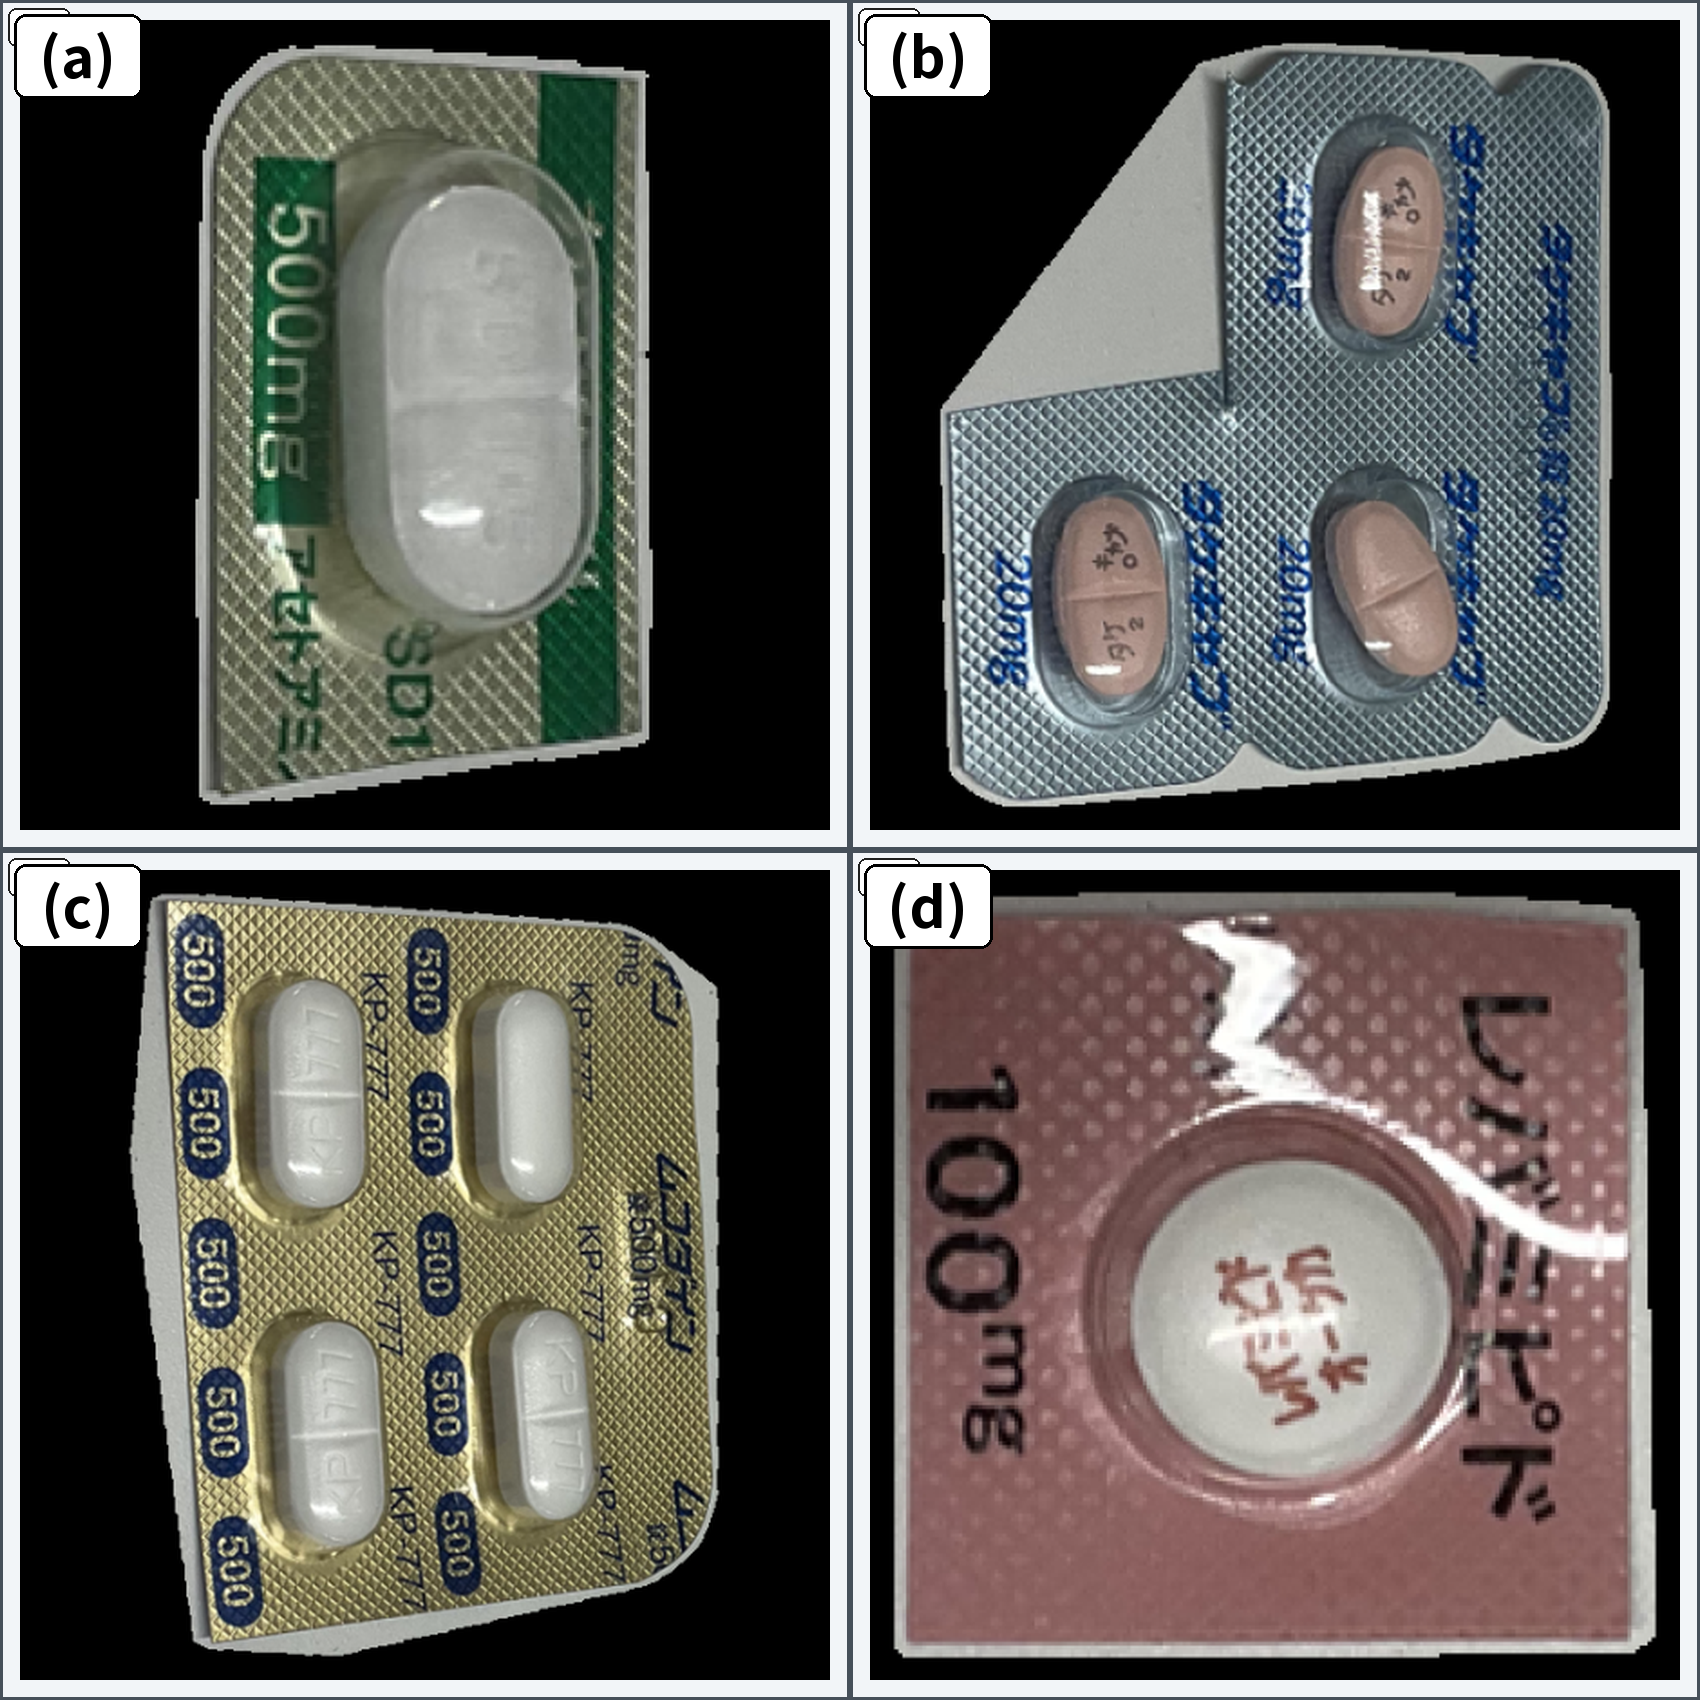
\includegraphics[width=0.78\linewidth]{figures/generated_ver10/condition_d_errors_2x2.png}
  \caption[主条件Dの代表的な誤分類モデル入力]{主条件Dの代表的な誤分類モデル入力．
  （a）IMG\_0027：カロナール錠500mg$\rightarrow$デエビゴ錠5mg，
  （b）IMG\_0047：タケキャブ錠20mg$\rightarrow$ジャディアンス錠10mg，
  （c）IMG\_0236：ムコダイン錠500mg$\rightarrow$レボチロキシンNa錠50$\mu$g，
  （d）IMG\_0020：レバミピド錠100mg$\rightarrow$プレドニン錠5mgである．
  著者が保存済みモデル入力を再配置した．}
  \label{fig:condition_d_errors}
\end{figure}

表\ref{tab:condition_d_errors}と図\ref{fig:condition_d_errors}に7件の内訳と代表4件を示す．
7件はすべて表面で，残存錠数は1錠2件，3錠2件，4錠2件，6錠1件であった．
正解側ではムコダイン錠500mgが2件，ほか5薬剤が各1件であった．
予測先ではデエビゴ錠5mgが3件，ほか4薬剤が各1件であり，41クラス外文字列はなかった．
ただし，誤分類が7件と少なく，包装の向き，錠数または印字が原因であるとは断定できない．
条件Cは，ver4の4条件の中では，単剤Top-1，画像単位完全一致率，領域ラベル一致率の3指標のすべてで最も高かった．
条件Cは条件Bに対し，単剤Top-1が2.44パーセントポイント，画像単位完全一致率が9.00パーセントポイント上昇した．
ただし，条件Cは全条件の結果を確認した後に選んだ探索的な最良条件であった．
このため，条件Cを事前に選んだ独立な確認実験の結果とは扱わなかった．

\begin{figure}[H]
  \centering
  \begin{tikzpicture}
    \begin{axis}[
      xbar,
      width=13.2cm,
      height=6.8cm,
      xmin=0,
      xmax=115,
      xtick={0,20,40,60,80,100},
      xlabel={正解率（\%）},
      symbolic y coords={D,C,B,A},
      ytick=data,
      bar width=7pt,
      tick label style={font=\small},
      label style={font=\small},
      legend style={
        at={(0.5,1.12)},
        anchor=south,
        legend columns=3,
        font=\small,
        draw=none
      },
      reverse legend,
      nodes near coords={\pgfmathprintnumber[fixed,zerofill,precision=2]{\pgfplotspointmeta}\%},
      every node near coord/.append style={font=\scriptsize,anchor=west,xshift=1pt},
      enlarge y limits=0.15,
      xmajorgrids=true
    ]
      \addplot[fill=blue!60,draw=blue!80!black] coordinates {(94.77,A) (96.17,B) (98.61,C) (97.56,D)};
      \addplot[fill=orange!70,draw=orange!80!black] coordinates {(76.75,A) (80.00,B) (89.00,C) (82.75,D)};
      \addplot[fill=green!55,draw=green!60!black] coordinates {(94.22,A) (95.22,B) (97.33,C) (95.83,D)};
      \legend{単剤Top-1精度,画像単位完全一致率,領域ラベル一致率}
    \end{axis}
  \end{tikzpicture}
  \caption{条件AからDの評価結果（3指標）}
  \label{fig:condition_comparison}
\end{figure}

\subsection{収集画像学習ver5}

ver5では，ver4条件Dを基準とし，全41クラスへ表面中央の縦2分割画像と縦4分割画像を各1枚追加した．
基画像は1,265枚から1,347枚へ増加した．
ver4条件Cを基準とした後継実験ではなかった．
結果を表\ref{tab:web_v5}に示した．

\begin{table}[H]
  \centering
  \caption{収集画像学習ver5の評価結果}
  \label{tab:web_v5}
  \scriptsize
  \begin{tabular}{|c|p{5.0cm}|r|r|r|}
    \hline
    実験 & 内容 & 単剤Top-1 & \shortstack{画像単位\\完全一致} & \shortstack{領域ラベル\\一致} \\ \hline
    ver5-1 & ver4条件D基準，1,265基画像 & 280/287（97.56\%） & 331/400（82.75\%） & 1,725/1,800（95.83\%） \\ \hline
    ver5-2 & 1,347基画像，5エポック & 281/287（97.91\%） & 348/400（87.00\%） & 1,745/1,800（96.94\%） \\ \hline
    ver5-3 & 1,347基画像，総提示数をver5-1と一致 & 281/287（97.91\%） & 356/400（89.00\%） & 1,755/1,800（97.50\%） \\ \hline
  \end{tabular}
\end{table}

単剤Top-1は，追加前のver5-1に対してver5-2，ver5-3とも1枚の増加であった．
薬剤をクラスタとしたブートストラップ95\%区間は$-2.02$から$+2.57$パーセントポイント，McNemar検定の$p$値は1.00であり，単剤精度の明確な改善は確認されなかった．
合成複数薬剤画像ではver5-2，ver5-3がver5-1を上回ったが，黒背景のタイル合成複数薬剤画像に限られる結果であった．
ver5-3がver4条件Cと同じ89.00\%を示しても，基準条件と学習画像が異なるため，同一モデルまたは再現結果とは扱わなかった．

\subsection{収集画像学習ver6（LoRA容量の探索的追試）}\label{sec:ver6_training}

ver6は，ver4条件Cと同じ評価画像287枚ならびに合成複数薬剤画像400枚・1,800領域で評価した．
評価入力の一覧が両条件で同一であることを確認したため，同じ評価集合に対する結果として比較した．

ver6では，ver4条件CからLoRAのランク$r$を16から32へ増やし，$\alpha/r=2.0$を保つため，スケーリング係数$\alpha$も32から64へ比例変更した．
これに伴い，学習可能パラメータ数は21,233,664から42,467,328へ約2倍となった．
モデル重みのデータ型であるBF16，学習対象層，基画像1,265枚，17種類の提示条件，5エポック，延べ提示画像数107,525枚，実効バッチサイズ128，乱数シード42は，すべてver4条件Cと同一であった．
変更の主眼はLoRA容量に置いた．
ただし，$r$と$\alpha$の2設定値を変更したため，容量増加の因果効果だけを証明する設計ではなかった．

\begin{table}[H]
  \centering
  \caption{ver4条件Cとver6の評価結果（評価集合は同一）}
  \label{tab:condition_c_ver6}
  \scriptsize
  \begin{tabular}{|c|p{3.6cm}|r|r|r|}
    \hline
    条件 & LoRA設定 & 単剤\mbox{Top-1} & \shortstack{画像単位\\完全一致} & \shortstack{領域ラベル\\一致} \\ \hline
    ver4条件C & ランク16，係数32，学習可能21,233,664パラメータ & 283/287（98.61\%） & 356/400（89.00\%） & 1,752/1,800（97.33\%） \\ \hline
    ver6 & ランク32，係数64，学習可能42,467,328パラメータ & 286/287（99.65\%） & 374/400（93.50\%） & 1,773/1,800（98.50\%） \\ \hline
  \end{tabular}
\end{table}

ver4条件Cとver6の評価結果を表\ref{tab:condition_c_ver6}に示した．
単剤予測の対応は，両条件とも正解282枚，条件Cだけ正解1枚，ver6だけ正解4枚，両条件とも誤り0枚であった．
McNemar検定（正確法）は両側$p=0.375$であり，条件Cに対する有意な改善は確認されなかった．
ver6は収集画像学習の探索条件内で単剤Top-1の最高観測値を示したため，探索的追試として詳述した．
ただし，ver6は全条件の結果確認後に選択した条件であった．
実行前の主条件はver4条件Dであった．
また，乱数シード42による1回の観測だけであったため，LoRA容量増加の効果と再現性は確認できなかった．

\subsection{ver6の単剤評価}\label{sec:ver6_single}

ver6は，薬剤部で撮影した評価画像287枚中286枚を正しく識別した．
単剤Top-1精度は99.65\%であり，画像単位の参考値として算出したWilson法による95\%信頼区間は98.05\%から99.94\%であった．
同一薬剤内の画像は相互に独立とは限らないため，この区間を287個の独立標本に基づく外部性能の区間とは解釈しなかった．
薬剤別正解率のマクロ平均は99.73\%であった．
表面は211/212枚，99.53\%，裏面は75/75枚，100.00\%，フルシートは29/29枚，100.00\%であった．
錠数別では，残存錠数が4錠の画像だけが44枚中43枚であり，ほかはすべて100.00\%であった．

条件Cで誤分類した4件について，ver6では表\ref{tab:condition_c_errors_resolved}のとおり4件すべてを正しく識別した．
そのうち，条件Cがムコダイン錠500mgに対して生成した「ケコダイン錠500mg」は学習対象の41クラスに存在しない文字列であったが，ver6ではこの文字列を生成しなかった．

\begin{table}[H]
  \centering
  \caption{条件Cの誤分類4件に対するver6の予測}
  \label{tab:condition_c_errors_resolved}
  \scriptsize
  \setlength{\tabcolsep}{2pt}
  \begin{tabular}{|p{3.2cm}|p{2.7cm}|c|c|p{2.7cm}|p{2.9cm}|}
    \hline
    画像ID & 正解薬剤 & 面 & 錠数 & 条件Cの予測 & ver6の予測 \\ \hline
    IMG\_0027 & カロナール錠500mg & 表 & 1 & デエビゴ錠5mg & カロナール錠500mg（正解） \\ \hline
    IMG\_0234 & ムコダイン錠500mg & 表 & 4 & ケコダイン錠500mg & ムコダイン錠500mg（正解） \\ \hline
    IMG\_0238 & ムコダイン錠500mg & 表 & 6 & デエビゴ錠5mg & ムコダイン錠500mg（正解） \\ \hline
    IMG\_0042 & メチコバール錠500$\mu$g & 表 & 5 & メトクロプラミド錠5mg & メチコバール錠500$\mu$g（正解） \\ \hline
  \end{tabular}
\end{table}

\begin{figure}[H]
  \centering
  \includegraphics[width=0.78\linewidth]{figures/generated_ver10/condition_c_vs_ver6_errors_2x2.png}
  \caption[条件Cとver6で正誤が変化したモデル入力]{条件Cとver6で正誤が変化した保存済みモデル入力．
  （a）IMG\_0236：正解ムコダイン錠500mg，条件Cは正解，ver6はレボフロキサシン錠500mg，
  （b）IMG\_0234：正解ムコダイン錠500mg，条件Cはケコダイン錠500mg，ver6は正解，
  （c）IMG\_0027：正解カロナール錠500mg，条件Cはデエビゴ錠5mg，ver6は正解，
  （d）IMG\_0042：正解メチコバール錠500$\mu$g，条件Cはメトクロプラミド錠5mg，ver6は正解である．
  著者が保存済みモデル入力を再配置した．}
  \label{fig:condition_c_vs_ver6}
\end{figure}

図\ref{fig:condition_c_vs_ver6}に，条件Cからver6で正誤が変化した4件を示す．
条件Cの4件をver6が正解した一方，ver6は条件Cが正解したIMG\_0236を誤分類した．
改善方向は一様ではなく，単一乱数シードのため再現性を確認していない．
ムコダイン錠500mgで複数の変化が観測されたが，事例数が少なく原因は特定できない．
また，「ケコダイン錠500mg」は41クラス外の生成文字列である．

一方，ver6は条件Cが正解していた別の1件を誤分類した．
表\ref{tab:single_errors}にver6の誤分類を示した．

\begin{table}[H]
  \centering
  \caption{ver6の誤分類}
  \label{tab:single_errors}
  \small
  \begin{tabular}{|p{3.8cm}|p{3.5cm}|p{3.8cm}|c|c|}
    \hline
    画像ID & 正解薬剤 & 予測薬剤 & 面 & 錠数 \\ \hline
    IMG\_0236 & ムコダイン錠500mg & レボフロキサシン錠500mg & 表 & 4 \\ \hline
  \end{tabular}
\end{table}

ムコダイン錠500mgは，条件Cとver6の双方で誤分類が集中した薬剤であった．
ただし，ver6の誤分類は計1件だけであり，原因を統計的に特定できるだけの事例数はなかった．

なお，初期実画像方式の保存済み条件のうち，17種拡張・640画素・実効バッチ8の5分割交差検証は286/287（99.65\%）であり，ver6と同数であった．
17種拡張・実効バッチ2の保存済み条件は285/287（99.30\%）であった．
以下の画像別対応比較は11種提示条件の283/287を対象としたものであり，初期実画像方式の最良保存条件に対するver6の優越を示すものではなかった．
初期実画像方式の11種拡張による5分割交差検証は283/287枚，ver6は286/287枚を正しく識別した．
ただし，両者は学習元と評価設計が異なるため，以下は同一画像に対する予測の探索的な参考比較であった．
方式間の優越性を検定する確認的比較ではなかった．
画像識別子を正規化して287件すべてを一意に対応させた結果を表\ref{tab:paired_initial_web}に示した．

\begin{table}[H]
  \centering
  \caption{初期実画像方式とver6の画像別対応}
  \label{tab:paired_initial_web}
  \small
  \begin{tabular}{|l|r|}
    \hline
    対応 & 画像数 \\ \hline
    両方式とも正解 & 282 \\ \hline
    ver6のみ正解 & 4 \\ \hline
    初期実画像方式のみ正解 & 1 \\ \hline
    両方式とも誤分類 & 0 \\ \hline
  \end{tabular}
\end{table}

不一致対は4対1であり，McNemar検定（正確法）は両側$p=0.375$であった．
有意差は認められず，ver6の優越を証明した結果ではなかった．

収集画像を学習元としたver6は，学習には使用していない薬剤部の写真287枚で99.65\%を得た．
この結果から，RTI，部分画像，画像拡張およびLoRA設定を組み合わせた構成で，41クラスの識別を実行できることを探索的に確認した．
ただし，新しい薬剤へ同程度の性能で拡張できることまでは示さなかった．

\subsection{追加学習していないQwen3.5-4Bとの比較}\label{sec:qwen_baseline}

LoRAを適用していないQwen3.5-4Bの保存済み予測を287件すべて再集計した．
追加学習していないQwen3.5-4Bは，41クラスの薬剤名をそのままの形では出力できなかった．
保存時の包含判定では3/287（1.05\%，Wilson 95\%信頼区間0.36--3.03\%）であった．
一方，本報告書の厳密一致では0/287（0.00\%，Wilson 95\%信頼区間0.00--1.32\%）であった．
保存時に成功とされた3件も薬剤名を含む説明文であり，要求した薬剤名だけの出力形式には一致しなかった．
同一287画像に対する3系列の集計を表\ref{tab:qwen_baseline}に示した．

\begin{table}[H]
  \centering
  \caption{追加学習していないQwen3.5-4B，ver4条件D，ver6の同一287画像による比較}
  \label{tab:qwen_baseline}
  \small
  \begin{tabular}{|p{4.6cm}|r|r|p{3.1cm}|}
    \hline
    保存系列 & 厳密一致 & Top-1精度 & Wilson 95\%信頼区間 \\ \hline
    追加学習していないQwen3.5-4B & 0/287 & 0.00\% & 0.00--1.32\% \\ \hline
    ver4条件D & 280/287 & 97.56\% & 95.05--98.81\% \\ \hline
    探索的ver6 & 286/287 & 99.65\% & 98.05--99.94\% \\ \hline
  \end{tabular}
\end{table}

追加学習していない側とLoRAを適用した側では，入力の前処理，入力画像サイズ，実行環境および出力の制御が異なる．
このため，観測された差はLoRAの有無だけを変更した比較ではなく，保存済みの実行全体の差である．
LoRAだけの効果は確認しておらず，入力条件をそろえた再比較が必要である．
正誤が異なった画像は条件Dに対して280件，ver6に対して286件であり，すべて一方向へ偏った．
このため，McNemar検定の$p$値は画像別の対応を記述する参考値であり，モデルの優越性を示す根拠としては用いない．

\subsection{Gemini 3.5 Flashとの対応比較}\label{sec:gemini_compare}

保存済みのGemini 3.5 Flashによる予測とver6の予測を，同じ評価画像287枚について対応付けた．
薬剤名と画像ファイル名を結合した識別子は287件すべてで一意に一致し，元画像と正解ラベルの不一致もなかった．
ただし，過去にGemini APIへ送信したJPEG変換後のバイト列は保存されておらず，実際の送信入力そのものは検証できなかった．

Gemini 3.5 Flashは284/287枚（98.95\%），ver6は286/287枚（99.65\%）を正しく識別した．
差はver6が0.70パーセントポイント高かった．
画像別の正誤対応を表\ref{tab:paired_gemini_ver6}に示した．

Gemini 3.5 Flashとver6で正誤が異なった画像を表\ref{tab:discordant_gemini_ver6}に示した．
\begin{table}[H]
  \centering
  \caption{Gemini 3.5 Flashとver6の画像別正誤対応}
  \label{tab:paired_gemini_ver6}
  \small
  \begin{tabular}{|l|r|r|}
    \hline
     & Gemini正解 & Gemini誤分類 \\ \hline
    ver6正解 & 283 & 3 \\ \hline
    ver6誤分類 & 1 & 0 \\ \hline
  \end{tabular}
\end{table}

不一致対はver6のみ正解が3件，Geminiのみ正解が1件であった．
式\eqref{eq:mcnemar_exact}による正確McNemar検定の両側$p$値は0.625であり，有意差は認められなかった．
ただし，不一致対は4件だけであり，検出力は低かった．
この結果は，両方式の統計的同等性を示すものではなかった．

\begin{table}[H]
  \centering
  \caption{Gemini 3.5 Flashとver6で正誤が異なった画像}
  \label{tab:discordant_gemini_ver6}
  \scriptsize
  \begin{tabular}{|p{1.8cm}|p{4.2cm}|p{4.2cm}|}
    \hline
    画像ID & Gemini 3.5 Flashの予測 & ver6の予測 \\ \hline
    IMG\_0095 & タケキャブ錠10mg（誤り） & デエビゴ錠5mg（正解） \\ \hline
    IMG\_0236 & ムコダイン錠500mg（正解） & レボフロキサシン錠500mg（誤り） \\ \hline
    IMG\_0044 & タケキャブ錠20mg（誤り） & メチコバール錠500$\mu$g（正解） \\ \hline
    IMG\_0045 & メトクロプラミド錠5mg（誤り） & メチコバール錠500$\mu$g（正解） \\ \hline
  \end{tabular}
\end{table}

Geminiの保存実験では，元画像を最大589,824画素へ縮小し，JPEG品質90へ変換したうえで，41クラスの候補一覧をプロンプトへ与えていた．
一方，ver6では背景除去後の448画素正方形画像を用いた．
入力前処理，プロンプト，推論方式が異なるため，本比較は各保存済みパイプライン全体の探索的参考比較とした．
また，Geminiのモデルリビジョン，温度，乱数シードは記録されておらず，API再実行による完全な再現はできなかった．

\subsection{ver6の合成複数薬剤画像評価}\label{sec:ver6_multi}

ver6は，合成複数薬剤画像400枚中374枚を画像単位完全一致で識別した．
画像単位完全一致率は93.50\%であり，参考値として算出したWilson法による95\%信頼区間は90.65\%から95.53\%であった．
検出された領域数は，正解領域数と同じ1,800件であった．
保存順の貪欲な一対一対応では，正解ラベル1,800件中1,773件が予測ラベルと対応した．
厳密一致による再集計でも，これらの件数は変わらなかった．
領域ラベル一致率は98.50\%であり，独立性を仮定した参考値として算出したWilson法による95\%信頼区間は97.83\%から98.97\%であった．
400枚は，単剤実写真を黒い間隔を空けてタイル状に配置して作成した．
ただし，各領域がどの単剤写真に由来するかは記録されていない．
このため，使用した元写真の総数，除外画像，元写真ごとの再利用回数は再集計できなかった．
単剤実写真を再利用した合成評価であるため，単剤評価から独立に取得した検証とは扱わなかった．
領域ラベル一致率98.50\%は，単剤Top-1精度99.65\%とは異なる独立標本に対する外部評価ではなかった．
両者の差は，タイル合成と領域抽出という処理を経たことによる劣化を含んでいた．
また，元写真の対応記録がないため，1,800領域を独立標本として扱わなかった．

図\ref{fig:multi_count}に薬剤数別の完全一致率を示した．
2薬剤では96.00\%，3薬剤では95.00\%，5薬剤では93.00\%，8薬剤では90.00\%であった．
画像内の薬剤数が増えるにつれて，完全一致率は低下した．
画像単位完全一致は，画像内のすべての領域が正しく識別された場合にのみ成立する指標である．
したがって，1画像当たりの領域数が増えるほど，完全一致の成立条件は厳しくなる．
ただし，各薬剤数の評価枚数は100枚であり，薬剤数間の差の有意性は検定していない．

\begin{figure}[H]
  \centering
  \begin{tikzpicture}
    \begin{axis}[
      ybar,
      width=13.2cm,
      height=6.5cm,
      ymin=0,
      ymax=105,
      ytick={0,20,40,60,80,100},
      ylabel={画像単位完全一致率（\%）},
      xlabel={画像内の薬剤数},
      symbolic x coords={2,3,5,8},
      xtick=data,
      bar width=30pt,
      tick label style={font=\small},
      label style={font=\small},
      nodes near coords={\pgfmathprintnumber[fixed,precision=0]{\pgfplotspointmeta}\%},
      nodes near coords align={vertical},
      every node near coord/.append style={font=\normalsize\bfseries},
      ymajorgrids=true,
      enlarge x limits=0.16
    ]
      \addplot[fill=blue!55,draw=blue!80!black] coordinates {(2,96) (3,95) (5,93) (8,90)};
    \end{axis}
  \end{tikzpicture}
  \caption{ver6における薬剤数別の完全一致率}
  \label{fig:multi_count}
\end{figure}

本評価では，薬剤部で撮影した元写真を黒い隙間で区切って格子状に配置した合成複数薬剤画像を用いた．
薬剤の重なり，影，手やトレーの写り込み，反射，複雑な背景を含まなかった．
したがって，93.50\%を薬剤部で撮影する実画像の性能として解釈できなかった．
複数薬剤の実用性能を判断するには，実際の撮影条件による独立評価が必要であった．

\subsection{収集画像学習ver7（探索的追加実験）}\label{sec:ver7_results}

ver7は，ver6およびver4条件Cと同じ評価画像287枚ならびに合成複数薬剤画像400枚・1,800領域で評価した．
ver7では，ver4条件Cから次の3点を同時に変更した．
\begin{enumerate}
  \item 表面中央の縦2分割画像と縦4分割画像を41クラスへ各1枚追加し，基画像を1,265枚から1,347枚へ増やした．
  \item 延べ提示画像数を107,525枚から114,495枚へ増やした．
  \item 推論を自由生成から，学習マニフェスト由来の41候補の中で平均トークン対数尤度が最大のものを選ぶ方式へ変更した．
\end{enumerate}
LoRAはランク16，スケーリング係数32であり，ver4条件Cと同一であった．
したがって，ver6との比較では，画像追加，延べ提示画像数，推論方式に加え，LoRAのランクと係数も異なった．
なお，ver7の来歴記録には基画像数1,265枚という変更前の値が残る一方，設定，学習マニフェストおよび実ファイルは1,347枚で一致した．
このため，来歴記録は更新漏れのある補助資料として扱い，基画像数の根拠には用いない．

\begin{table}[H]
  \centering
  \caption{ver6とver7の評価結果（評価集合は同一）}
  \label{tab:ver6_ver7}
  \scriptsize
  \begin{tabular}{|c|p{4.5cm}|r|r|r|}
    \hline
    条件 & 主な変更点 & 単剤\mbox{Top-1} & \shortstack{画像単位\\完全一致} & \shortstack{領域ラベル\\一致} \\ \hline
    ver6 & LoRAランク32，係数64 & 286/287（99.65\%） & 374/400（93.50\%） & 1,773/1,800（98.50\%） \\ \hline
    ver7 & 基画像1,347枚，総提示114,495，41候補から選択 & 284/287（98.95\%） & 380/400（95.00\%） & 1,780/1,800（98.89\%） \\ \hline
  \end{tabular}
\end{table}

ver6とver7の評価結果を表\ref{tab:ver6_ver7}に示した．
ver7は画像単位完全一致380/400（95.00\%），領域ラベル一致1,780/1,800（98.89\%）であり，複数薬剤の2指標ではver6を上回った．
一方，単剤Top-1は284/287（98.95\%）であり，ver6を下回った．
41候補から選ぶ推論による正解数の増加は認められず，同じアダプタによる自由生成の予測と完全に一致した．
ver4条件Cからは3要因，ver6からはLoRA容量を含む4要因が異なるため，結果の変化を個別要因へ帰属できなかった．
ver6は単剤Top-1，ver7は合成複数薬剤の2指標で高い値を示しており，探索的追試の中でも単一の条件がすべての指標で最良とはならなかった．
ver6，ver7とも乱数シード42による1回の学習結果であり，条件間の差の再現性は確認しなかった．

\subsection{収集画像学習ver8・ver9の単剤評価}\label{sec:ver8_ver9_results}

ver8とver9は，単剤経路と複数薬剤経路を分けた2経路パッケージとして保存されている．
本節では，本報告書の主指標である単剤側だけを扱う．

両条件とも，BF16 LoRA，ランク32，スケーリング係数64，学習対象層はq，k，v，o射影およびgate，up，down射影であり，
学習可能パラメータ数は42,467,328であった．
基画像は1,347枚であり，延べ提示画像数はver6と同じ107,525枚へ固定した．
エポック数5，学習率$2.0\times10^{-4}$，実効バッチサイズ128，乱数シード42は，ver6と同一であった．
ver9はver8に対し，17提示条件のうち明度倍率1.0の条件を，複数領域の解像度劣化を模擬する条件へ置き換えた点だけが異なる．

ここで注意すべき点として，保存された2経路パッケージの単剤経路は，
新たに学習したver8・ver9のアダプタではなく，保存済みver6アダプタをそのまま用いる設定であった．
実際，パッケージの単剤経路の予測は，画像ID，正解薬剤，予測薬剤および正誤の4項目について，
ver6の保存済み予測287件と不一致0件で完全に一致した．
したがって，パッケージとしての単剤結果はver6の結果の再掲であり，ver6を上回る単剤性能を示すものではなかった．

一方，ver8・ver9のアダプタ自身を同じ評価画像287枚へ適用した診断値は，
いずれも286/287（99.65\%）であった．
この値はver6と同数であるが，誤分類した画像は条件ごとに異なった．
ver8はIMG\_0130（正解エンレスト錠200mg，表，残存4錠）をフロセミド錠200mgと予測した．
この予測文字列は，フロセミド錠20mgとは含量が異なり，学習対象の41クラスには存在しなかった．
ver9はIMG\_0236（正解ムコダイン錠500mg，表，残存4錠）をレボフロキサシン錠500mgと予測し，
これはver6が誤分類した画像および予測先と同一であった．

保存済みの昇格判定では，単剤性能の維持を示す項目だけが真であり，
ver6およびver7の複数薬剤性能を上回る項目と，総合的な昇格の可否を示す項目はいずれも偽であった．
したがって，ver8とver9は性能退行のない候補条件であり，採用条件として昇格したものではない．

収集画像学習ver1からver9までの単剤Top-1精度を表\ref{tab:ver1_ver9_single}にまとめた．
すべて同じ評価画像287枚に対する値である．

\begin{table}[H]
  \centering
  \caption{収集画像学習ver1からver9の単剤Top-1精度（評価はいずれも同じ287枚）}
  \label{tab:ver1_ver9_single}
  \scriptsize
  \setlength{\tabcolsep}{3pt}
  \begin{tabular}{|l|p{5.6cm}|r|r|}
    \hline
    条件 & 主な設定・変更点 & 基画像数 & 単剤Top-1 \\ \hline
    ver1 & RTIと1錠区画，4ビットQLoRA，ランク8，q/v射影 & 457 & 259/287（90.24\%） \\ \hline
    ver2 & 表裏を分離し，面別の部分画像を追加 & 451 & 255/287（88.85\%） \\ \hline
    ver3 & 異なる錠剤セル，縦2分割・縦4分割を追加 & 1,265 & 281/287（97.91\%） \\ \hline
    ver4条件A & ver3設定を基準に4ビットQLoRAを再構成 & 1,265 & 272/287（94.77\%） \\ \hline
    ver4条件B & BF16 LoRAへ変更（量子化等を同時に変更） & 1,265 & 276/287（96.17\%） \\ \hline
    ver4条件C & ランク16・係数32，学習対象層を拡大 & 1,265 & 283/287（98.61\%） \\ \hline
    \textbf{ver4条件D} & \textbf{撮影変動対応の重複しない17提示条件（主条件）} & 1,265 & \textbf{280/287（97.56\%）} \\ \hline
    ver5-1 & ver4条件Dを基準とする再実行 & 1,265 & 280/287（97.56\%） \\ \hline
    ver5-2 & 表面中央の縦2分割・縦4分割画像を追加 & 1,347 & 281/287（97.91\%） \\ \hline
    ver5-3 & 総提示数をver5-1へ一致させた条件 & 1,347 & 281/287（97.91\%） \\ \hline
    ver6 & ランク32・係数64へ増加（探索的追試） & 1,265 & 286/287（99.65\%） \\ \hline
    ver7 & 基画像1,347枚，41候補から選ぶ推論へ変更 & 1,347 & 284/287（98.95\%） \\ \hline
    ver8$^{\ast}$ & 2経路構成，ランク32，延べ提示数をver6へ固定 & 1,347 & 286/287（99.65\%） \\ \hline
    ver9$^{\ast}$ & ver8の明度1.0条件を解像度劣化条件へ置換 & 1,347 & 286/287（99.65\%） \\ \hline
  \end{tabular}

  \vspace{1mm}
  {\scriptsize $^{\ast}$ ver8・ver9の値は各アダプタ自身を単剤評価した診断値である．
  2経路パッケージの単剤経路は保存済みver6アダプタを用いるため，パッケージとしての単剤結果はver6と同一である．}
\end{table}

表\ref{tab:ver1_ver9_single}では，ver6，ver8およびver9が286/287で同数の最高観測値であった．
したがって，収集画像学習の探索条件の中で，ver6だけが単独の最高条件ではなかった．
ただし，ver8とver9はいずれもver6と同じランク32・係数64を用いており，
基画像数と提示条件だけが異なる派生条件である．
また，各条件は乱数シード42による1回の学習結果であり，同じ287枚を反復使用した評価である．
このため，286/287という同数の観測から，条件間の優劣および再現性を判断することはできなかった．

\subsection{黒い区切りのない合成画像による予備評価}

\subsubsection{ver3入力素材を用いた領域抽出だけの評価}\label{sec:zero_gap_detection}

黒い隙間への依存を切り分ける追試として，収集画像学習ver3で保存した448 $\times$ 448の背景除去済みQwen入力素材を，継ぎ目のない共通背景へ非接触で配置した．
5薬剤，6薬剤，8薬剤を各3枚，合計9枚生成し，正解薬剤数や正解外接矩形を処理へ与えずに領域を抽出した．
図\ref{fig:gapless_detection}に5薬剤画像の入力と検出結果の構成を模式的に示した．

\begin{figure}[H]
  \centering
  \begin{tikzpicture}[
    canvas/.style={draw,minimum width=6.2cm,minimum height=3.9cm,fill=cyan!12},
    item/.style={draw,rounded corners=1mm,fill=white,minimum width=1.0cm,minimum height=1.45cm,font=\scriptsize},
    detection/.style={draw=green!55!black,very thick,minimum width=1.25cm,minimum height=1.75cm}
  ]
    \node[canvas] (input) {};
    \node[item] at ([xshift=-2.0cm,yshift=0.8cm]input.center) {包装1};
    \node[item] at ([xshift=0cm,yshift=0.9cm]input.center) {包装2};
    \node[item] at ([xshift=2.0cm,yshift=0.7cm]input.center) {包装3};
    \node[item] at ([xshift=-1.0cm,yshift=-1.0cm]input.center) {包装4};
    \node[item] at ([xshift=1.2cm,yshift=-1.0cm]input.center) {包装5};
    \node[font=\small, below=1mm of input] {入力：共通背景上へ非接触で配置};

    \node[canvas, right=0.8cm of input] (output) {};
    \node[item] at ([xshift=-2.0cm,yshift=0.8cm]output.center) {};
    \node[item] at ([xshift=0cm,yshift=0.9cm]output.center) {};
    \node[item] at ([xshift=2.0cm,yshift=0.7cm]output.center) {};
    \node[item] at ([xshift=-1.0cm,yshift=-1.0cm]output.center) {};
    \node[item] at ([xshift=1.2cm,yshift=-1.0cm]output.center) {};
    \node[detection] at ([xshift=-2.0cm,yshift=0.8cm]output.center) {1};
    \node[detection] at ([xshift=0cm,yshift=0.9cm]output.center) {2};
    \node[detection] at ([xshift=2.0cm,yshift=0.7cm]output.center) {3};
    \node[detection] at ([xshift=-1.0cm,yshift=-1.0cm]output.center) {4};
    \node[detection] at ([xshift=1.2cm,yshift=-1.0cm]output.center) {5};
    \node[font=\small, below=1mm of output] {出力：画像から決定した5領域};
  \end{tikzpicture}
  \caption{黒い区切りのない合成画像に対する領域抽出の模式図}
  \label{fig:gapless_detection}
\end{figure}

採点用正解領域57件に対して57領域を抽出し，領域の重なり率（Intersection over Union：IoU）0.25以上で57件すべてが対応した．
個数と全領域が一致した画像は9/9枚であった．
図\ref{fig:zero_gap_gapless_actual}に，本節の保存済み9枚のうち\texttt{8薬剤\_gapless\_01}の入力と検出結果を示した．

\begin{figure}[H]
  \centering
  \includegraphics[width=\linewidth]{figures/generated_ver10/zero_gap_gapless_example.png}
  \caption[共通背景・非接触配置における入力と領域抽出結果の実例]{共通背景・非接触配置における入力と領域抽出結果の実例（\texttt{8薬剤\_gapless\_01}）．
  （a）は採点用期待領域8件の入力，（b）は保存済みの検出枠である．
  検出器へ正解薬剤数，正解外接矩形および薬剤名は与えておらず，8領域を検出してIoU 0.25以上で8件すべてが対応した．
  入力はver3の背景除去済み448 $\times$ 448素材を共通背景上へ非接触配置した合成画像であり，実写の自然配置画像ではない．
  著者が保存済み入力と検出結果を再配置した．}
  \label{fig:zero_gap_gapless_actual}
\end{figure}

図\ref{fig:zero_gap_gapless_actual}は，模式図\ref{fig:gapless_detection}の後段に対応する実出力である．
包装同士が離れ，背景色が一様であるため，前景マスクの連結成分が包装単位で分離した．
ただし，これは色の安定した共通背景上で包装同士を離した合成複数薬剤画像による領域抽出だけの確認であり，Qwenによる薬剤名推論は実施しなかった．
したがって，この9/9を条件Cの複数薬剤完全一致率89.00\%と置き換えることはできなかった．
また，実際の机上背景，接触，重なり，影を含む自然画像での検出性能も示さなかった．

\subsubsection{元写真タイルを用いたver6・ver7の検出後識別}\label{sec:zero_gap_identification}

これとは別に，評価用の元写真を背景除去せず，余白と間隔を0画素としてタイル配置した合成画像を用いた．
薬剤数が5，6，8の画像を各3枚，合計9枚生成し，正解薬剤数を検出器へ与えずに領域検出と薬剤名推論を行った．
入力には，元写真全体を縦横比を保って各タイルへ縮小した画像を用いた．
この条件は，固定400枚の黒背景キャッシュとは異なっていた．
結果を表\ref{tab:zero_gap_end_to_end}に示した．

\begin{table}[H]
  \centering
  \caption{黒い区切りのない未知個数画像9枚に対する探索的評価}
  \label{tab:zero_gap_end_to_end}
  \small
  \setlength{\tabcolsep}{4pt}
  \begin{tabular}{|c|c|c|c|c|c|}
    \hline
    条件 & \shortstack{薬剤名と個数の\\完全一致} & \shortstack{薬剤名の種類の\\完全一致} & \shortstack{期待\\ラベル数} & 検出数 & \shortstack{対応した\\正解ラベル} \\ \hline
    ver6 & 2/9（22.22\%） & 2/9（22.22\%） & 57 & 66 & 55/57（96.49\%） \\ \hline
    ver7 & 2/9（22.22\%） & 3/9（33.33\%） & 57 & 66 & 55/57（96.49\%） \\ \hline
  \end{tabular}
\end{table}

「薬剤名と個数の完全一致」は，画像ごとに薬剤名とその個数がすべて一致した画像数を9枚中の比率で示した．
「薬剤名の種類の完全一致」は，個数を無視して薬剤名の種類だけが一致した画像数を9枚中の比率で示した．
「対応した正解ラベル」は，画像内の予測と正解を薬剤名と個数で照合できた個数を，期待57領域に対する比率で示した．
この値は，検出枠の位置の正しさを測る指標ではない．
両条件とも期待領域数57件に対して66領域を検出し，検出数は期待数を9件上回った．
過検出の例を図\ref{fig:zero_gap_flush_actual}に示した．

\begin{figure}[H]
  \centering
  \includegraphics[width=\linewidth]{figures/generated_ver10/zero_gap_flush_example.png}
  \caption[元写真タイルにおける入力と検出結果の過検出例]{元写真タイルにおける入力と検出結果の過検出例（\texttt{5薬剤\_flush\_02}）．
  （a）は採点用期待領域5件の入力，（b）は保存済みの検出枠である．
  検出器へ正解薬剤数，配置，薬剤名およびタイル寸法は与えておらず，8領域を検出して3件を過検出した．
  過検出した3件は，いずれも左端タイルの元写真の周辺部に写り込んだ被写体に対応した．
  入力は背景除去を行わない元写真を余白・間隔0画素でタイル配置した合成画像であり，実写の自然配置画像ではない．
  著者が保存済み入力と検出結果を再配置した．}
  \label{fig:zero_gap_flush_actual}
\end{figure}

正解ラベル55件がいずれかの予測と対応しても，検出数とラベル多重集合の双方が一致した画像は2/9枚にとどまった．
これは9枚だけの合成画像による探索的評価であり，固定400枚の結果と直接比較できなかった．
また，元写真を接触させたタイル境界は含むが，包装同士の重なり，任意の机上配置，手やトレーの写り込みを含む自然画像ではなかった．

\subsection{条件Cの信頼ゲート評価}\label{sec:trust_gate_results}

本節はver4条件Cのアダプタに対する予備評価であり，探索的追試ver6に対して信頼ゲートを評価したものではない．
ver6の信頼ゲート性能は本研究では評価しなかった．
条件Cのモデルに対し，校正集合だけで決定した信頼ゲートを最終評価集合へ適用した．
系列スコアのしきい値は$\tau_s=-0.011180272$，候補間マージンのしきい値は$\tau_m=0.282711724$とした．
11視点のTTA多数決一致率のしきい値は$\tau_a=0.636363636$（11視点中7件以上の一致）とし，第1候補とTTA多数決の薬剤名一致を必須とした．
これらのしきい値は，最終評価集合の推論開始前に固定した．

表\ref{tab:trust_gate_phase}に校正集合と最終評価集合の結果を示した．
校正集合では，既知薬剤139枚中137枚に回答し，誤回答は0件であった．
未知薬剤67枚では64枚を保留し，危険通過は3件であった．
最終評価集合では，既知薬剤148枚に対するゲート適用前の第1候補正解は145枚であった．
ゲート適用後は134枚に回答し，回答した134枚はすべて正解であった．
ゲートは適用前の誤回答3枚をすべて保留したが，適用前に正しかった11枚も保留した．

\begin{table}[H]
  \centering
  \caption{条件Cの信頼ゲートにおける校正集合と最終評価集合の結果}
  \label{tab:trust_gate_phase}
  \small
  \begin{tabular}{|l|r|r|r|r|}
    \hline
    評価段階 & 既知薬剤への回答 & 既知誤回答 & 未知薬剤の保留 & 危険通過 \\ \hline
    校正集合 & 137/139 & 0 & 64/67 & 3 \\ \hline
    最終評価集合 & 134/148 & 0 & 50/58 & 8 \\ \hline
  \end{tabular}
\end{table}

最終評価集合における既知薬剤への回答率は90.54\%であり，Wilson法による95\%信頼区間は84.75\%から94.28\%であった．
回答した既知薬剤の正解率は100.00\%であり，Wilson法による95\%信頼区間は97.21\%から100.00\%であった．
一方，未知薬剤の保留率は86.21\%であり，Wilson法による95\%信頼区間は75.07\%から92.84\%であった．
既知薬剤と未知薬剤のいずれにも，同一製品に由来する複数画像が含まれていた．
そのため，これらは画像単位の参考区間であり，製品単位で独立な外部性能の区間ではなかった．
未知薬剤58枚中8枚（13.79\%）に既知薬剤名を回答した．
危険通過は校正集合の3/67（4.48\%）から最終評価集合の8/58（13.79\%）へ悪化し，校正集合で観測された水準は再現されなかった．

表\ref{tab:trust_gate_unsafe}に，信頼ゲートを通過した未知薬剤と，誤って回答した既知薬剤との組合せを示した．
アラセプリル錠25mgとアテノロール錠25mgは，いずれもアルダクトンA錠25mgとして各2枚が通過した．
そのほか4薬剤で各1枚が通過した．

\begin{table}[H]
  \centering
  \caption{信頼ゲートを通過した未知薬剤と誤って回答した既知薬剤との組合せ}
  \label{tab:trust_gate_unsafe}
  \small
  \begin{tabular}{|p{5.0cm}|p{5.0cm}|r|}
    \hline
    未知薬剤 & 回答した既知薬剤 & 枚数 \\ \hline
    アラセプリル錠25mg「日医工」 & アルダクトンA錠25mg & 2 \\ \hline
    アテノロール錠25mg「NIG」 & アルダクトンA錠25mg & 2 \\ \hline
    アテノロール錠50mg「NIG」 & ムコダイン錠500mg & 1 \\ \hline
    アロプリノール錠100mg「NIG」 & プロマックD錠75mg & 1 \\ \hline
    エゼチミブ錠10mg「日医工」 & エソメプラゾールカプセル20mg & 1 \\ \hline
    プレガバリンカプセル150mg「日医工」 & プレドニン錠5mg & 1 \\ \hline
  \end{tabular}
\end{table}

危険通過8件の元画像パスとモデル入力パスは最終評価マニフェストから一意に復元できた．
ただし，未知薬剤は外部Web収集画像であり，各画像の本文転載条件までは確認できなかったため，
指示書の掲載条件に従って実画像図は掲載しない．
また，既知側と未知側で取得条件が異なり，外観だけから誤り原因を断定できない．

今回の最終評価集合では，厳密な薬剤名照合，TTA，系列スコア，候補間マージンだけでは，未知薬剤の危険通過を十分に防止できなかった．
また，既知薬剤は薬剤部で撮影した評価画像，未知薬剤は収集画像であり，画像の取得条件および被写体の占有範囲が異なった．
したがって，本評価は信頼ゲートの予備評価であり，実画像の未知薬剤を安全に検出できることを示す外部評価ではなかった．
信頼ゲートは完成していないと判断した．

\subsection{総合考察}

条件比較では，4ビット量子化，勾配チェックポイント，マイクロバッチ構成を同時に変更した条件Bが条件Aを上回った．
さらに，LoRAのランク，スケーリング係数，適用層を同時に変更した条件Cが条件Bを上回った．
各比較で複数要因を同時に変更したため，BF16化または追加学習対象層の拡大だけの効果とは解釈できなかった．
ver6は，$\alpha/r=2.0$を保ったままランク$r$を2倍にし，それに伴って$\alpha$を比例変更した．
学習可能パラメータ数は21,233,664から42,467,328へ約2倍となり，単剤Top-1は283/287（98.61\%）から286/287（99.65\%）へ増加した．
対応比較のMcNemar検定は両側$p=0.375$であった．
乱数シード42による1回の観測だけであったため，LoRA容量増加の効果と再現性は確認できなかった．

本報告書で主結果として扱うver4条件Dの単剤Top-1は97.56\%であり，ver6の99.65\%は収集画像学習の探索条件内で全条件の結果確認後に得た最高観測値であった．
ただし，ver8およびver9のアダプタも同じ286/287（99.65\%）であり，ver6は収集画像学習内でも単独の最高条件ではなかった．
さらに，初期実画像方式の保存済み最良条件E12bも286/287（99.65\%）であった．
ver8とver9の2経路パッケージの単剤経路は保存済みver6アダプタを用いる設定であり，ver6を上回る単剤性能を示すものではなかった．
ver7では，画像単位完全一致率が95.00\%，領域ラベル一致率が98.89\%となり，両指標でver6を上回った．
一方，単剤Top-1は98.95\%であった．
したがって，ver6を確認的な主結果または全指標で最良の条件とは扱わなかった．
次の評価では，主条件を事前に固定し，新しく撮影した画像だけで確認する必要がある．

Gemini 3.5 Flashとの対応比較では，ver6が0.70パーセントポイント高かった．
しかし，正確McNemar検定の両側$p$値は0.625であり，有意差は認められなかった．
不一致対は4件だけであり，方式間の統計的同等性を示す結果でもなかった．
また，入力前処理，プロンプト，推論方式が異なるため，差をモデル本体だけへ帰属できなかった．

追加学習していないQwen3.5-4Bは，41クラスの薬剤名をそのままの形では出力できなかった．
保存時の包含判定では3/287，厳密一致では0/287であった．
条件Dおよびver6との差は大きかったが，追加学習していない側は素画像，LoRAを適用した条件は前処理後の画像を用いた．
また，追加学習していない側のモデルリビジョンと実行環境の記録は残っていなかった．
したがって，本比較は追加学習の必要性を検討する参照情報にはなるが，
LoRAだけの因果効果または提案手法の優越性を示す対照実験とは扱えなかった．

ver6の評価画像287枚では誤分類が1件となった．
一方，複数薬剤では領域ラベル一致率が98.50\%であっても，8薬剤の完全一致率は90.00\%まで低下した．
画像単位完全一致では，領域ごとの誤りが画像全体の不一致として反映される．
したがって，複数薬剤では単剤モデルの改善に加え，検出結果の検証と保留機構が必要であった．

条件Cの信頼ゲートは，既知薬剤の誤回答3件をすべて保留し，回答した134件はすべて正解であった．
一方で，正しく識別できていた11件も保留し，未知薬剤8件を危険通過させた．
未知薬剤保留率は，校正集合の64/67（95.52\%）から最終評価集合の50/58（86.21\%）へ低下した．
このことから，生成系列スコアとTTA一致率は，外観が類似する未知薬剤に対して十分な安全指標ではなかった．
この結果は条件Cのアダプタに対する予備評価であり，ver6の信頼ゲート性能を示すものではなかった．
PTP包装の印字を光学文字認識（Optical Character Recognition：OCR）で読み取り，薬剤名と含量を候補と照合するなど，モデル出力とは独立した根拠を導入する必要があると考えた．

\subsection{妥当性の限界}

本実験の限界を，データ，評価設計，統計，再現性，比較対象および実運用の6区分に整理した．

{\small
\begin{enumerate}
\setlength{\itemsep}{0pt}
  \item \textbf{データ：}評価対象は41クラスに限られた．収集画像42枚のうち32枚は現行の収集記録と直接照合でき，残る10枚も削除前の収集記録から出典候補を確認した．ただし，その10枚は元画像から現存画像までの加工の履歴をたどれなかった．
  \item \textbf{評価設計：}評価287枚は収集画像学習ver1からver9のLoRA学習には使用していないが，研究初期の実画像方式では一部を学習へ使用した．同じ287枚を収集画像学習の条件検討に反復使用し，条件選択後の新規評価専用集合を設けなかった．ver6，ver8およびver9はいずれも結果確認後に得た条件である．合成複数薬剤画像は単剤写真を再利用し，黒い隙間を含むため，実写複数薬剤の性能を示さなかった．黒い区切りのない画像も9枚だけであった．
  \item \textbf{統計：}各条件は乱数シード42による1回だけであり，学習のばらつきを評価しなかった．McNemar検定では画像対間の独立性を確認できず，薬剤または撮影元をクラスタとする方式差の区間推定も行わなかった．1,265枚の基画像と1,800領域は相関を含むため，独立標本として扱わなかった．
  \item \textbf{再現性：}CUDAの決定論的アルゴリズムを無効にしており，実行コードのバージョンも実行記録に残っていなかった．合成複数薬剤画像の記録には各領域の元写真の対応がなく，再利用回数を再集計できなかった．収集画像と実行結果の一部はバージョン管理の対象外であり，報告書のディレクトリだけでは再学習できなかった．
  \item \textbf{比較対象：}追加学習していないQwen3.5-4Bの保存結果は再集計したが，素画像を入力した実験であり，LoRAを適用した条件と入力の前処理をそろえていなかった．同じ入力によるOCRと薬剤辞書の照合や，単純な画像分類器も評価していない．Geminiとの比較も入力の前処理と推論方式が異なり，提案構成の優越性を示す比較ではなかった．
  \item \textbf{実運用：}収集画像の整理と実画像の撮影に要した工数を測定しなかった．信頼ゲートは条件Cだけで評価し，未知薬剤の危険通過が3/67から8/58へ悪化した．既知側と未知側の取得条件も異なったため，安全な保留，新しい薬剤への一般化および臨床利用可能性を示さなかった．
\end{enumerate}
}

%----------------------------------------------------------------------
\clearpage
\section{結論・今後の課題}\label{sec:conclusion}
%----------------------------------------------------------------------

\subsection{結論}

本研究では，収集したPTP包装のフルシート表面・裏面画像からRTIと部分画像を生成し，
Qwen3.5-4BをLoRAで追加学習したうえで，学習には使用していない近畿大学病院薬剤部で撮影した写真287枚を用いて，
41クラスのTop-1識別性能を評価した．

主結果として扱うver4条件Dは287枚中280枚を正しく識別し，Top-1精度97.56\%を得た．
同条件の合成複数薬剤画像400枚では，画像単位完全一致率82.75\%，領域ラベル一致率95.83\%であった．
結果を確認した後の探索的な追試では，ver6が286/287，ver7が284/287であり，ver8・ver9のアダプタもver6と同じ286/287であった．
ただし，これらはいずれも結果を見た後に選んだ条件であり，条件Cとの対応比較でも有意差は認められなかったため，確認的な主結果ではない．
Gemini 3.5 Flashの保存予測は284/287であり，追加学習していないQwen3.5-4Bは41クラスの薬剤名をそのままの形では出力できなかった．
ただし，方式間では入力の前処理と出力の制御が異なるため，これらの差はモデル本体の優劣を示すものではない．

複数薬剤では，黒い区切りを設けた合成画像400枚でver6が374枚を正しく識別した．
一方，黒い区切りのない9枚では，薬剤名と個数がすべて一致した画像は2枚にとどまった．
条件Cの信頼ゲートは，回答した既知薬剤134枚をすべて正しく識別したが，未知薬剤58枚中8枚に既知薬剤名を答えた．

以上より，フルシートの表面1枚と裏面1枚を学習元とし，RTIと部分画像を自動生成する構成で，
41クラスのPTP包装を識別できることを確認した．
残存錠数や切り出し範囲ごとに学習用写真を個別に撮影する必要はなくなったが，
収集，撮影および前処理を含む総作業時間は比較しておらず，作業負担の削減量は確認していない．
また，各条件は乱数シード42による1回の学習であり，同じ287枚を条件検討に反復使用した．
このため，新しく撮影した写真による確認，複数の乱数シードによる再現性の確認，
RTIと部分画像それぞれの寄与の切り分け，実際に撮影した複数薬剤画像の評価，
および未知薬剤への回答を安全に保留する仕組みは，いずれも今後の課題である．

\subsection{今後の課題}

今後は，対象とする薬剤の数を増やすとともに，間違った薬剤を答えないようにしていく．
薬剤の数を増やす際は，学習用の写真と評価用の写真を薬剤部で別々に撮影し，
評価用の写真は学習にはいっさい使わずに識別性能を確認する．
間違った薬剤を答えないようにするには，41クラス以外の薬剤が入力された場合に回答を保留する仕組みが必要である．
本研究の信頼ゲートでは，生成時のスコアとTTAの一致率だけでは未知薬剤の誤回答を防げなかった．
このため，PTP包装の印字をOCRで読み取り，
モデルが答えた薬剤名と一致しない場合は回答を保留する方法を検討する．

\clearpage

\section*{謝辞}
\addcontentsline{toc}{section}{謝辞}

本研究の遂行にあたり，多大なご指導とご助言を賜った森山真光准教授に，心より感謝申し上げます．
また，本研究で用いた薬剤画像の撮影にご協力いただくとともに，薬剤鑑別に関する貴重なご助言を賜った共同研究者である近畿大学病院薬剤部の皆様，ならびに木村裕一教授に深く感謝申し上げます．

\clearpage
\addcontentsline{toc}{section}{参考文献}

{\footnotesize
\raggedright
\bibliographystyle{junsrt}
\bibliography{260731}
}

\end{document}
